\documentclass[a4paper]{article}
\usepackage[english]{babel}
\usepackage[utf8]{inputenc}
\usepackage[left=3.0cm, right=3.0cm]{geometry}
\usepackage{amsmath}
\usepackage{graphicx}
\usepackage{fancyhdr}
\usepackage{hyperref}
\usepackage{enumerate}
\usepackage{amssymb}
\usepackage{amsthm}
\usepackage{tikz-cd}
\usepackage{pdfpages}

\DeclareMathOperator*{\argmax}{arg\,max}
\DeclareMathOperator*{\argmin}{arg\,min}

\newcommand{\R}{\mathbb{R}}
\newcommand{\Z}{\mathbb{Z}}
\newcommand{\N}{\mathbb{N}}
\newcommand{\C}{\mathbb{C}}
\newcommand{\Q}{\mathbb{Q}}
\newcommand{\F}{\mathbb{F}}
\newcommand{\E}{\mathbb{E}}
\renewcommand{\P}{\mathbb{P}}
\newcommand{\f}[1]{\text{#1}}
\newcommand{\MLE}{\text{MLE}}
\newcommand{\MAP}{\text{MAP}}

\newcommand{\<}{\langle}
\renewcommand{\>}{\rangle}
\renewcommand{\^}{\wedge}
\renewcommand{\v}{\vee}



\newcommand{\Nor}{\mathcal{N}}



\pagestyle{fancy}
\fancyhf{}
\lhead{\today}
\chead{EECS 126}
\rhead{Albert Zhang}
\cfoot{\thepage}

\makeatletter
\renewcommand{\@seccntformat}[1]{}
\makeatother

% \setcounter{secnumdepth}{0}
\setlength{\parindent}{0pt}
\setlength{\parskip}{8pt}
\setlength{\textheight}{635pt}

\title{\textbf{EECS 126 -- Probability \& Random Processes}}
\author{\large Taught by K. Ramchandaran \\
Notes \& Exercises by Albert Zhang}
\date{Spring 2019}

\begin{document}

\maketitle
\tableofcontents
\newpage

%%%%%%%%%%%%%%%%%%%% 
\section{Homework 1}

\begin{enumerate}
    \item (i) By principle of inclusion exclusion, we know that the probability of event $A$ or event $B$ happening is $\P[A] + \P[B] - \P[A \cap B]$. Since this includes the probability that both $A$ and $B$ happen, we subtract $\P[A \cap B]$ to obtain $\P[A] + \P[B] - 2\P[A \cap B]$.
    
    (ii) If $A$ is independent of itself, then we have $\P[A \mid A] = \P[A]$. But if $A$ occurs, then we know that $A$ occurs, thus $\P[A \mid A] = 1$ if the chance of $A$ occurring is strictly positive. In this case $\P[A] = 1$. Else, if $A$ has zero chance of occurring, i.e. $\P[A] = 0$, then $\P[A \mid A] = 0$ since $A$ never occurs in the first place. It follows that $A$ is independent of itself in this case. Thus, if $A$ is independent of itself, then $\P[A]$ must equal either 0 or 1.
    
    \item Let $B$ be the random variable denoting the number of heads among Bob's first $n$ coins, and $A$ be the random variable denoting the number of heads among Alice's first $n$ coins. Then the probability that Bob flips more heads out of his $n + 1$ coins than Alice flips out of her $n$ coins is
    \begin{align*}
        \P[B > A] + \frac{1}{2}\P[A = B] &= \frac{1}{2}(2\P[B > A] + \P[A = B]) \\
            &= \frac{1}{2}(\P[B > A] + \P[A > B] + \P[A = B]) \\
            &= \frac{1}{2}(1) \\
            &= \frac{1}{2}.
    \end{align*}
    This follows since $\P[A > B] = \P[B > A]$ by symmetry.
    
    \item We proceed by induction on $k$. When $k = 1$, it is clear that the probability that the last ball is white is just $\frac{w}{w + b}$.
    
    Now suppose for some $k > 0$, the probability of the last ball being white is $\frac{w}{w + b}$. Then the probability that the last ball being black is $1 - \frac{w}{w + b} = \frac{b}{w + b}$. If we add the $(k+1)$th jar, then the probability of the last ball (in the $(k + 1)$th jar after one of the balls was moved from the $k$th jar) being white is
    \begin{align*}
     &\left(\frac{w}{w + b}\right)\left(\frac{w + 1}{w + b + 1}\right) + \left(\frac{b}{w + b}\right)\left(\frac{w}{w + b + 1}\right) \\
    &= \frac{w(w + b + 1)}{(w + b)(w + b + 1)} \\
    &= \frac{w}{w + b}.
    \end{align*}
    It follows then that for any $k > 0$, the probability that the last ball is white is $\frac{w}{w + b}$.
    
    \item Given a fixed $N$, denote $X_i$ the event that $i$ at least $i$ people get their assigned seat. Then applying principle of inclusion exclusion, we obtain the probability that nobody gets their assigned seat:
    \begin{align*}
        \P[X_0] - \P[X_1] + \P[X_2] - \dots \pm \P[X_N] &= \frac{1}{N!}\left(N! - \binom{N}{1}(N - 1)! + \binom{N}{2}(N - 2)! - \dots \pm 1\right) \\
        &= \sum\limits_{i = 0}^N \frac{(-1)^i\binom{N}{i}(N - i)!}{N!} \\
        &= \sum\limits_{i = 0}^N(-1)^i\frac{1}{i!}.
    \end{align*}
    Since the taylor expansion of $e^x$ is $\sum_{i = 0}^\infty \frac{x^i}{i!}$, if we take the limit as $N \to \infty$, then we see that our desired probability is just $e^{-1}$, or $\frac{1}{e}$.
    
    \item WLOG, let the cities be ranked by their number: $\{1, 2, \dots, N - 1, N\}$ (so the worst city is 1, the best city is $N$). We will sum the probabilities indexed by the cases where city $N$ is in the $i$th position for $i \in \{m + 1, m + 2, \dots, N - 1, N\}$. Since the probability of city $N$ being in position $i$ is $\frac{1}{N}$, and the probability of the highest ranking city among the first $i - 1$ cities being placed among the first $m$ positions is $\frac{m}{i - 1}$, we have the summation
    \begin{align*}
        \sum\limits_{i = m + 1}^N \frac{1}{N} \cdot \frac{m}{i - 1} &= \frac{m}{N}\sum\limits_{i = m + 1}^N \frac{1}{i - 1} \\
        &\approx \frac{m}{N}(\f{ln}(N) - \f{ln}(m)).
    \end{align*}
    Now, to find $m$ such that this probability is maximized, we differentiate over $m$ to obtain
    \begin{align*}
        \frac{\f{ln}N}{N} - \frac{\f{ln}m}{N} - \frac{1}{N} &= 0 \\
        \f{ln}N - \f{ln}m - 1 &= 0 \\
        \f{ln}m &= \f{ln}\frac{N}{e} \\
        m &= \frac{N}{e},
    \end{align*}
    as an approximation for the probability maximizing value of $m$ in terms of $N$.
    
    \item Denote the score by $(c, s)$ where $0 \leq c \leq n$ is the captain's score and $0 \leq s \leq m$ is superman's score. We can think of each sequence of baskets as paths of an $m \times n$ grid, with $(0, 0)$ and $(n, m)$ at opposite corners. There are a total of $\binom{m + n}{n}$ such paths with no restrictions. Now, the probability that the captain scores first given $n$ and $m$ is 
    \[
        \frac{\binom{m + n - 1}{n - 1}}{\binom{m + n}{n}} = \frac{\frac{(m + n - 1)!}{m!(n - 1)!}}{\frac{(m + n)!}{m!n!}} = \frac{n}{m + n},
    \]
    since there are $\binom{m + n - 1}{n - 1}$ paths from $(1, 0)$ to $(n, m)$. Similarly, the probability (which is just the complement of the above) of superman scoring first is $\frac{m}{m + n}$. Now, in the probability that the captain scores first, there is some chance that there will be a tie later on. Consider the first instance $(k, k)$ they tie after captain scores the first point. Given that the sequence goes through $(k, k)$, we find that the conditional probability of superman scoring first and captain scoring first is the same, by symmetry. Therefore, we can just reflect the sequence across the diagonal, producing a bijection between sequences starting with $(0, 0) - (1, 0)$ and resulting in a tie somewhere down the line and sequences starting with $(0, 0) - (0, 1)$ and ending at $(n, m)$. It follows that within the probability that captain scores first, the probability that we don't want (i.e. the probability that there is a tie somewhere down the line) is just the probability of superman scoring first, $\frac{m}{n + m}$. Thus, the probability of the captain always being strictly ahead of superman is
    \[
        \frac{n}{n + m} - \frac{m}{n + m} = \frac{n - m}{n + m}.
    \]
    
\end{enumerate}
\section{Homework 2}

\begin{enumerate}
    \item \textbf{Packet Routing}
    
    (a) Let $S$ be the random variable counting the number of arriving packets in the time interval $[0, 1]$, and let $X$ be the random variable counting the number of packets routed to $A$. We will show that $X$ is poisson distributed with parameter $\lambda p$. We compute the probability that $X = k$ as a summation based on the number of packets that arrive at the switch:
    \begin{align*}
        \P[X = k] &= \sum\limits_{i = k}^\infty \P[S = i]\binom{i}{k}(1 - p)^{i - k}p^k \\
            &= \sum\limits_{i = k}^\infty \frac{e^{-\lambda}\lambda^i}{i!}\binom{i}{k}(1 - p)^{i - k}p^k \\
            &= \frac{\lambda^k p^k e^{-\lambda}}{k!}\sum\limits_{j = 0}^\infty \frac{\lambda^j(1 - p)^j}{j!} \\
            &= \frac{\lambda^k p^k e^{-\lambda}e^{\lambda(1 - p)}}{k!} \\
            &= \frac{e^{-\lambda p}(\lambda p)^k}{k!} \sim \f{Poisson}(\lambda p).
    \end{align*}
    
    (b) Consider $\P[A = k | B = 0]$. This is equal to $\P[S = k]p^k = e^{-\lambda}\frac{\lambda^k}{k!}p^k$, that is, the probability that $k$ packets arrive at the switch and all $k$ of these packets are routed to $A$. However, by our result from part (a), $\P[A = k] = e^{-\lambda p}\frac{(\lambda p)^k}{k!}$. Thus, the number of packets routed to $A$ and the to $B$ cannot be independent since
    \[
    \P[A = k | B = 0] = e^{-\lambda}\frac{\lambda^k}{k!}p^k \neq e^{-\lambda p}\frac{(\lambda p)^k}{k!} = \P[A = k].
    \]
    
    \item \textbf{Compact Arrays}
    
    Note that $X = i - (\f{\# of 0's that appear before ith index})$. We can separate the second portion into i.i.d. indicator random variables $I_1, \dots, I_{i - 1}$, where $I_k$ indicates whether a 0 appears in the $k$th position or not. Then we have that
    \begin{align*}
    \E[X] &= \E[i - (\f{\# of 0's that appear before ith index})] \\
        &= i - \E[I_1 + \dots + I_{i - 1}] \\
        &= i - (i - 1)\E[I_1] \\
        &= i - (i - 1)\frac{1}{10} \\
        &= \frac{9i + 1}{10}.
    \end{align*}
    Now, we calculate the variance, using the same indicator variables and the property that they are mutually independent and identically distributed:
    \begin{align*}
        \f{Var}(X) &= \f{Var}(i - (I_1 + \dots + I_{i - 1})) \\
            &= \f{Var}(I_1 + \dots + I_{i - 1}) \\
            &= \f{Var}(I_1) + \dots + \f{Var}(I_{i - 1}) \\
            &= (i - 1)(\E[I_1^2] - \E[I_1]^2) \\
            &= (i - 1)(\frac{1}{10} - \frac{1}{100}) \\
            &= \frac{9i - 9}{100}.
    \end{align*}
    
    \item \textbf{Message Segmentation}
    
    (a) First, we note that the support of our PMF $f$ is $(q, r)$ where $0 \leq r < m$ whenever $q > 0$ and $0 < r < m$ whenever $q = 0$ (since $N$ is strictly positive and $N = mq + r$) for integers $q$ and $r$. Let $N$ be the random variable of number of bytes in the message. Now, we find our PMF to be
    \begin{align*}
        f(q, r) &= \P[Q = q, R = r] \\
            &= \P[N = mq + r] \\
            &= (1 - p)^{mq + r - 1}p
    \end{align*}
    where $q$ and $r$ are restricted to the support mentioned above.
    
    (b) First, we compute the marginal PMF of $Q$ when $q > 0$:
    \begin{align*}
        \P[Q = q] &= \sum\limits_{i = 0}^{m - 1}\P[Q = q, R = i] \\
            &= \sum\limits_{i = 0}^{m - 1}(1 - p)^{mq + i - 1}p \\
            &= (1 - p)^{mq - 1}p\sum\limits_{i = 0}^{m - 1}(1 - p)^i \\
            &= (1 - p)^{mq - 1}p\left(\frac{1 - (1 - p)^m}{1 - (1 - p)}\right) \\
            &= (1 - p)^{mq - 1} - (1 - p)^{mq + m - 1}.
    \end{align*}
    Now, if $q = 0$, then we replace the starting index 0 with 1 and instead get:
    \begin{align*}
        \P[Q = 0] &= \sum\limits_{i = 1}^{m - 1}\P[Q = 0, R = i] \\
            &= \sum\limits_{i = 1}^{m - 1}(1 - p)^{i - 1}p \\
            &=p\left(\frac{1 - (1 - p)^{m - 1}}{1 - (1 - p)}\right) \\
            &= 1 - (1 - p)^{m - 1}
    \end{align*}
    
    On the other hand, we compute the marginal PMF of $R$ for $R = r > 0$:
    \begin{align*}
        \P[R = r] &= \sum\limits_{i = 0}^\infty \P[Q = i, R = r] \\
            &= \sum\limits_{i = 0}^\infty(1 - p)^{mi + r - 1}p \\ 
            &= (1 - p)^{r - 1}p\sum\limits_{i = 0}^\infty((1 - p)^m)^i \\
            &= \frac{p(1 - p)^{r - 1}}{1 - (1 - p)^m}
    \end{align*}
    
    Now, we compute the marginal PMF of $R$ when $R = 0$:
    \begin{align*}
        \P[R = 0] &= \sum\limits_{i = 1}^\infty \P[Q = i, R = 0] \\
            &= \sum\limits_{i = 1}^\infty(1 - p)^{mi - 1}p \\
            &= \frac{p}{1 - p}\left(\frac{(1 - p)^m}{1 - (1 - p)^m}\right) \\
            &= \frac{p(1 - p)^{m - 1}}{1 - (1 - p)^m}.
    \end{align*}
    
    (c) Now that we are given $N > m$, $q$ is at least 1, and our support becomes nicer and with less casework. That is, our support now consists of points $(q, r)$ for integers $q$ and $r$ that satisfy $q > 0$ and $0 \leq r < m$.
    
    The marginal PMF of $Q$ stays the same:
     \begin{align*}
        \P[Q = q] &= \sum\limits_{i = 0}^{m - 1}\P[Q = q, R = i] \\
            &= (1 - p)^{mq - 1} - (1 - p)^{mq + m - 1}.
    \end{align*}
    
    We compute the updated marginal PMF of $R$:
    \begin{align*}
        \P[R = r] &= \sum\limits_{i = 1}^\infty\P[Q = i, R = r] \\
        &= \sum\limits_{i = 1}^\infty(1 - p)^{mi + r - 1}p \\
        &= p(1-p)^{m + r - 1}\sum\limits_{i = 0}^\infty(1 - p)^{mi} \\
        &= \frac{p(1 - p)^{m + r - 1}}{1 - (1 - p)^m}.
    \end{align*}
    
    \item \textbf{Almost Fixed Points of a Permutation}
    
    We can split $X$ into indicator variables $I_1, \dots, I_n$ where $I_k$ indicates whether or not $k$ is almost a fixed point of a given permutation. Then since the probability of a number being almost a fixed point is just $\frac{3}{n}$ (3 possible "almost fixed points", the two adjacent points and itself), we get the expectation using linearity
    \begin{align*}
        \E[X] &= \E[I_1 + \dots + I_n] \\
            &= \E[I_1] + \dots + \E[I_n] \\
            &= n \cdot \frac{3}{n} \\
            &= 3.
    \end{align*}
    
    For variance, we must split our calculations into cases with respect to $n$.
    
    Case 1 ($n = 1$):
    The only permutation sends 1 to 1. Thus the variance is 0.
    
    Case 2 ($n = 2$):
    There are two permutations, both of which produce 2 almost fixed points. Thus the variance is 0 again.
    
    Case 3 ($n = 3$):
    There are six permutations, all of which produce 3 almost fixed points. Thus the variance is 0 again.
    
    Case 4: ($n = 4$):
    Look at case 5 first. The only changes we need to make are to the counting of $\sum_{k \neq j}\E[I_kI_j]$. First, if $k$ and $j$ are adjacent, the expectation stays the same, namely
    \[
        \frac{14}{n - 1} = \frac{14}{3}.
    \]
    Now, there are 4 ways such that $k$ and $j$ are two indices apart. WLOG consider points 1, 2, 3, 4, where $k = 1, j = 3$. Then there are 7 ways to assign an ordered pair so that 1 and 3 are almost fixed points: (1, 2), (1, 3), (1, 4), (2, 3), (2, 4), (4, 2), (4, 3). So the expectation for this case is 
    \[
        4 \cdot \frac{7}{n(n - 1)} = \frac{7}{3}.
    \]
    Adding everything up, we get
    \begin{align*}
        \f{Var}(X) &= \frac{14}{3} + \frac{7}{3} - 6 \\
            &= 1.
    \end{align*}
    
    
    Case 5 ($n > 4$): 
    We split our random variable $X$ into indicators $I_1, \dots, I_n$ where $I_k$ indicates whether or not $k$ is an almost fixed point. Then we can use linearity to get
    \begin{align*}
        \f{Var}(X) &= \E[X^2] - \E[X]^2 \\
            &= \E[(I_1 + \dots + I_n)^2] - 3^2 \\
            &= \E[(I_1^2 + \dots + I_n^2) + \sum_{k \neq j}I_kI_j] - 9 \\
            &= \sum_{i = 1}^n\E[I_i^2] + \sum_{k \neq j}\E[I_kI_j] - 9 \\
            &= n\left(\frac{3}{n}\right) + \sum_{k \neq j}\E[I_kI_j] - 9 \\
            &= \left(\sum_{k \neq j}\E[I_kI_j]\right) - 6.
    \end{align*}
    Now, to compute the expectations in the large parentheses, we must account for cases where $k$ and $j$ differ by: one index, two indices, more than two indices.
    
    (one index) There are $2n$ ways to choose $k$ and $j$ to produce this case. WLOG consider the four points 1, 2, 3, 4, where $j = 2, k = 3$. Then corresponding to points 2 and 3 we can assign 7 possible ordered pairs such that both are almost fixed points: (1, 2), (1, 3), (1, 4), (2, 3), (2, 4), (3, 2), (3, 4). Since there are $n(n-1)$ ways to assign any ordered pair, we have a probability of $\frac{7}{n(n-1)}$ for this case. Furthermore, the total expectation in this case would amount to
    \[
        2n \cdot \frac{7}{n(n-1)} = \frac{14}{n-1}.
    \]
    
    (two indices) Once again, there are $2n$ ways to choose $k$ and $j$ to produce this case. WLOG consider the five points 1, 2, 3, 4, 5, where $j = 2, k = 4$. Then corresponding to points 2 and 4 we can assign 8 possible ordered pairs such that both are almost fixed points: (1, 3), (1, 4), (1, 5), (2, 3), (2, 4), (2, 5), (3, 4), (3, 5). Similar to the previous case, the total expectation in this case would amount to
    \[
        2n \cdot \frac{8}{n(n-1)} = \frac{16}{n-1}.
    \]
    
    (more than two indices) Since there are $n(n-1)$ ways to pick any ordered pair of points, we subtract the previous two cases to get $n(n-1) - 4n = n^2 - 5n$ ways to choose $k$ and $j$ to produce this case. Since there is no interference between the two points, there would be $3\cdot3 = 9$ ways to assign almost fixed points. Therefore, the total expectation in this case would amount to
    \[
        (n^2 - 5n)\frac{9}{n(n-1)} = \frac{9n - 45}{n - 1}.
    \]
    
    Summing this all together, we get
    \begin{align*}
        \f{Var}(X) &= \frac{14}{n - 1} + \frac{16}{n - 1} + \frac{9n - 45}{n - 1} - 6 \\
            &= \frac{3n - 9}{n - 1} = 3 - \frac{6}{n - 1}.
    \end{align*}
    
    Now, noticing that the answers to case 3 and 4 satisfy the formula derived in case 5, we summarize:
    \[
    \f{Var}(X) = \begin{cases}
        0 & \f{ for } n = 1, 2, \\
        3 - \frac{6}{n - 1} & \f{ for } n > 2.
    \end{cases}
    \]
    
    \item \textbf{Introduction to Information Theory}
    
    (a) Using the definition, we have
    \begin{align*}
        H(X) &= -\sum_x p(x)\log p(x) \\
            &= -\sum_x \log \left(p(x)^{p(x)}\right) \\
            &= -\left(\log\left(\prod_x p(x)^{p(x)}\right)\right) \\
            &\geq 0,
    \end{align*}
    since the $0 \leq p(x) \leq 1$ for all $x$, and we have a product of terms between 0 and 1, of which the log will return a nonpositive real value, and negating gives us a nonnegative real value.
    
    (b) If $p = 1$ or $p = 0$, then the entropy would be 0. So intuitively, $p = 1/2$ should have a higher entropy than $p = 1/3$.
    
    For $p = 1/2$, we have
    \begin{align*}
        H(X) &= -\sum_{k = 0}^1 \frac{1}{2}\log_2\frac{1}{2} \\
            &= -\left(-\frac{1}{2} - \frac{1}{2}\right) \\
            &= 1.
    \end{align*}
    
    For $p = 1/3$, we have
    \begin{align*}
        H(X) &= -\left(\frac{1}{3}\log_2\frac{1}{3} + \frac{2}{3}\log_2\frac{2}{3}\right) \\
            &= -\left(\log_2\left(\left(\frac{1}{3}\right)^{\frac{1}{3}}\left(\frac{2}{3}\right)^{\frac{2}{3}}\right)\right) \\
            &= -\left(\log_2\left(\left(\frac{4}{27}\right)^{\frac{1}{3}}\right)\right) \\
            &\approx 0.9183...
    \end{align*}
    
    So the entropy when $p = 1/2$ is higher.
    
    (c) First, we see that
    \begin{align*}
        \P[Y = 0] &= \frac{1}{2}(1 - p_e) \\
        \P[Y = ~?] &= \frac{1}{2}(p_e) + \frac{1}{2}(p_e) = p_e \\
        \P[Y = 1] &= \frac{1}{2}(1 - p_e).
    \end{align*}
    
    Now, we compute the entropy, combining the cases where $Y = 0$ and $Y = 1$:
    \begin{align*}
        H(Y) &= -\left((1 - p_e)\log_2\left(\frac{1}{2}(1 - p_e)\right) + p_e\log_2p_e\right) \\
            &= -\left((1 - p_e)(-1 + \log_2(1 - p_e)) + \log_2\left(p_e^{p_e}\right)\right) \\
            &= 1 - p_e - \log_2\left((1 - p_e)^{1 - p_e}p_e^{p_e}\right).
    \end{align*}
    
    (d) First, we compute the probabilities at each point:
    \begin{align*}
        p(0, 0) &= \frac{1}{2}(1 - p_e) \\
        p(0, ?) &= \frac{1}{2}p_e \\
        p(1, 1) &= \frac{1}{2}(1 - p_e) \\
        p(1, ?) &= \frac{1}{2}p_e.
    \end{align*}
    
    Now, we compute the entropy, combining symmetric cases from above:
    \begin{align*}
        H(X, Y) &= -\left((1 - p_e)\log_2\left(\frac{1}{2}(1 - p_e)\right) + p_e\log_2\left(\frac{1}{2}p_e\right)\right) \\
            &= -\left((1 - p_e)(-1 + \log_2(1 - p_e)) + p_e(-1 + \log_2p_e)\right) \\
            &= 1 - \log_2\left((1 - p_e)^{1 - p_e}p_e^{p_e}\right).
    \end{align*}
    
    \item \textbf{Soliton Distribution}
    
    (a) The probability that a given degree $d$ packet is connected to the chunk we are about to peel off is
    \[
        \frac{\binom{N - k - 1}{d - 1}}{\binom{N - k}{d}} = \frac{\frac{(N - k - 1)!}{(d - 1)!(N - k - d)!}}{\frac{(N - k)!}{d!(N - k - d)!}} = \frac{d}{N - k}.
    \]
    Therefore, using linearity of expectation, the expected number of degree $d$ packets whose degrees will be reduced by one after removing the $(k + 1)$st packet should be 
    \[
    f_k(d) \cdot \frac{d}{N - k}.
    \]
    
    (b) For the $d = 1$ case, we have the following recurrence relation,
    \[
        f_{k + 1}(1) = f_k(2) \cdot \frac{2}{N - k},
    \]
    and if we plug in our desired $f_{k + 1}(1) = 1$ and formula $f_k(d) = (N - k)/[d(d - 1)]$, we see that the above recurrence relation holds:
    \[
        f_{k + 1}(1) = 1 = \frac{N - k}{2(1)} \cdot \frac{2}{N - k} = f_k(2) \cdot \frac{2}{N - k}.
    \]
    
    Now, for the general case where $d = 2,\dots,N$, we have the following recurrence relation,
    \[
        f_{k + 1}(d) = f_k(d + 1)\cdot\frac{d + 1}{N - k} + f_k(d)\cdot\left(1 - \frac{d}{N - k}\right),
    \]
    and if we plug in the formula $f_k(d) = (N - k)/[d(d - 1)]$, once again we see that the recurrence relation holds:
    \begin{align*}
        f_k(d + 1)\cdot\frac{d + 1}{N - k} + f_k(d)\cdot\left(1 - \frac{d}{N - k}\right) &= \frac{N - k}{d(d + 1)}\cdot\frac{d + 1}{N - k} + \frac{N - k}{d(d - 1)}\cdot\frac{N - k - d}{N - k} \\
            &= \frac{1}{d} + \frac{N - k - d}{d(d - 1)} \\
            &= \frac{N - (k + 1)}{d(d - 1)} \\
            &= f_{k + 1}(d),
    \end{align*}
    which is what we wanted. It follows that in order for $f_k(1) = 1$ to hold for $k = 0,\dots,N - 1$, we must have $f_k(d) = (N - k)/[d(d - 1)]$ for all $d = 2,\dots,N$.
    
    From this, we may deduce what $p(d)$ is for each $d > 1$. The probability of $p(d)$ for $d > 1$ satisfies $f_0(d) = N \cdot p(d)$. From the formula above, this gives us that $p(d) = \frac{1}{d(d-1)}$ for $d > 1$. For $d = 1$, we have $1 = f_1(1) = N \cdot p(1)$, which gives us $p(1) = \frac{1}{N}$.
    
    (c) We compute the expectation of $p(\cdot)$:
    \begin{align*}
        \E[p(\cdot)] &= \sum_{i = 1}^n d \cdot p(d) \\
            &= \frac{1}{n} + \sum_{i = 2}^n d \cdot \frac{1}{d(d-1)} \\
            &= \frac{1}{n} + \sum_{i = 2}^n \frac{1}{d - 1} \\
            &= \sum_{i = 1}^{n - 1}\frac{1}{i} \\
            &\approx \ln (n - 1),
    \end{align*}
    or just $\ln n$ for large $n$.
    
\end{enumerate}
\section{Homework 3}

\subsection{Graphical Density}
(a) We have
\[
2\cdot1\cdot A + 1\cdot1\cdot (2A) + 2\cdot1\cdot A = 1,
\]
so $A = \frac{1}{6}$. Below we sketch the p.d.f.'s for $f_X$, $f_Y$, and $f_{X|X+Y\leq3}$, respecitvely:

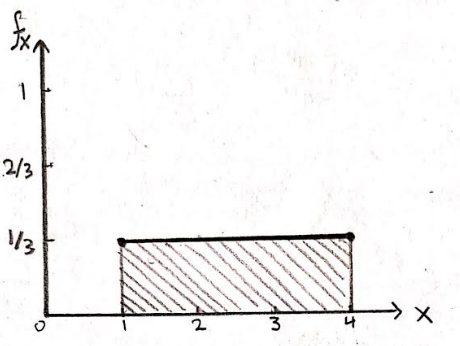
\includegraphics[scale=0.3]{f_X}
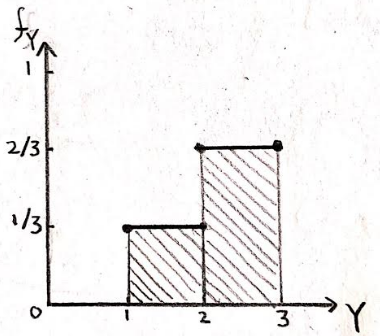
\includegraphics[scale=0.3]{f_Y}
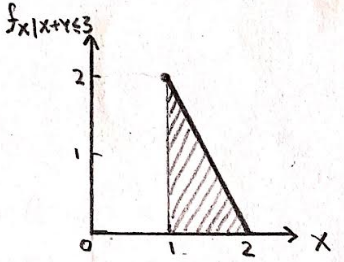
\includegraphics[scale=0.4]{f_conditional}

(b) For $\E[X|Y = y]$, we have symmetry on both $[1, 2]$ and $[2, 3]$ around $X = 2.5$. Thus $\E[X|Y = y] = 2.5$ for $1 \leq y \leq 3$.

On the other hand, for $\E[Y|X = x]$ is less symmetric, and we have the piecewise function:
\[
\E[Y|X = x] = 
\begin{cases}
    2 &\f{if } 1 \leq x \leq 2 \\
    2.5 &\f{if } 2 < x \leq 3 \\
    2 &\f{if } 3 < x \leq 4.
\end{cases}
\]

(c) From the previous part, we have $\E[X] = 5/2$, and $\E[Y] = (1/3)(2 + 5/2 + 2) = 13/6$. Now, we just need to find
\begin{align*}
    \E[XY] &= \int_1^3\int_1^2 \frac{xy}{6} dxdy + \int_2^3\int_2^3 \frac{xy}{3}dxdy + \int_1^3\int_3^4 \frac{xy}{6}dxdy \\
    &= 1 + \frac{25}{12} + \frac{7}{3} \\
    &= \frac{65}{12}.
\end{align*}
Thus we have that
\begin{align*}
\f{Cov}(X, Y) &= \E[XY] - \E[X]\E[Y] \\
&= \frac{65}{12} - \left(\frac{5}{2}\right)\left(\frac{13}{6}\right) \\
&= 0.
\end{align*}

\subsection{Conditional Distribution of a Poisson Random Variable with Exponentially Distributed Parameter}

(a) Integrating by parts, we get a recurrence relation, which we can exploit to get
\begin{align*}
    \E[\lambda^k] &= \int_0^\infty x^k f_\lambda(x) dx \\
    &= \int_0^\infty x^k\theta e^{-\theta x} dx \\
    &= \left.\left(-x^k e^{-\theta x}\right)\right|_{0 \f{ to } \infty} + \int_0^\infty kx^{k-1}e^{-\theta x} dx \\
    &= k\int_0^\infty x^{k-1}e^{-\theta x} dx \\
    &\quad\vdots \\
    &= \frac{k!}{\theta^{k-1}}\int_0^\infty e^{-\theta x} dx \\
    &= \frac{k!}{\theta^{k-1}}\left.\left(\frac{e^{-\theta x}}{-\theta}\right)\right|_{0 \f{ to } \infty} \\
    &= \frac{k!}{\theta^k},
\end{align*}
which is what we wanted.

(b) Using a similar approach to the previous part, we get an integral by parts and a recurrence relation which we exploit to get
\begin{align*}
    \P[X = k] &= \int_0^\infty e^{-x}\frac{x^k}{k!}f_\lambda(x) dx \\
    &= \frac{\theta}{k!}\int_0^\infty e^{-(\theta + 1)x}x^k dx \\
    &= \frac{\theta}{k!}\left(\left.\frac{-x^k e^{-(\theta + 1)x}}{\theta + 1}\right|_{o \f{ to } \infty} + \frac{k}{\theta + 1}\int_0^\infty x^{k-1}e^{-(\theta + 1)x} dx \right) \\
    &= \frac{\theta}{k!}\left(\frac{k}{\theta + 1}\int_0^\infty x^{k-1}e^{-(\theta + 1)x} dx \right) \\
    &\quad\vdots \\
    &= \frac{\theta}{k!}\left(\frac{k!}{(\theta + 1)^{k+1}}\right) \\
    &= \left(\frac{1}{\theta + 1}\right)^k\left(\frac{\theta}{\theta + 1}\right).
\end{align*}
Thus, $X$ is geometric (albeit shifted left by 1, i.e. with support $\N \cup \{0\}$) with parameter $p = \frac{\theta}{\theta + 1}$.

(c) Using Bayes' Rule and our result from the previous parts, we obtain:
\begin{align*}
    f_{\lambda|X}(\mu | X = k) &= \frac{f_\lambda(\mu) \cdot \P[X = k | \lambda = \mu]}{\P[X = k]} \\
    &= \frac{\left(\theta e^{-\theta\mu}\right)\left(e^{-\mu}\frac{\mu^k}{k!}\right)}{\left(\frac{1}{\theta + 1}\right)^k\left(\frac{\theta}{\theta + 1}\right)} \\
    &= \frac{e^{-(\theta + 1)\mu}\mu^k}{k!(\theta + 1)^{k+1}}.
\end{align*}

\subsection{Gaussian Densities}
(a) Let $Z = X_1 + X_2$. Then we have the convolution:
\begin{align*}
    f_Z(z) &= \int_{-\infty}^\infty f_{X_1}(t)f_{X_2}(z - t) dt \\
        &= \int_{-\infty}^\infty \frac{1}{\sigma_1\sigma_2 2\pi} e^{-\left(\frac{t^2}{2\sigma_1^2} + \frac{(z - t)^2}{2\sigma_2^2}\right)} dt \\
        &= \int_{-\infty}^\infty \frac{1}{\sqrt{2\pi}\sqrt{\sigma_1^2 + \sigma_2^2}} \cdot \frac{1}{\sqrt{2\pi}\frac{\sigma_1\sigma_2}{\sqrt{\sigma_1^2 + \sigma_2^2}}} e^{-\left(\frac{\sigma_2^2t^2 + \sigma_1^2t^2 - 2zt\sigma_1^2 + z^2\sigma_1^2}{2\sigma_1^2\sigma_2^2}\right)} dt \\
        &= \frac{1}{\sqrt{2\pi}\sqrt{\sigma_1^2 + \sigma_2^2}} \int_{-\infty}^\infty \frac{1}{\sqrt{2\pi}\frac{\sigma_1\sigma_2}{\sqrt{\sigma_1^2 + \sigma_2^2}}} e^{-\left(\frac{(\sigma_1^2 + \sigma_2^2)\left(t - \frac{\sigma_1^2z}{\sigma_1^2 + \sigma_2^2}\right)^2 - \frac{\sigma_1^4z^2}{\sigma_1^2 + \sigma_2^2} + z^2\sigma_1^2}{2\sigma_1^2\sigma_2^2}\right)} dt \\
        &= \frac{1}{\sqrt{2\pi}\sqrt{\sigma_1^2 + \sigma_2^2}} e^{-\frac{z^2}{2(\sigma_1^2 + \sigma_2^2)}}\int_{-\infty}^\infty \frac{1}{\sqrt{2\pi}\frac{\sigma_1\sigma_2}{\sqrt{\sigma_1^2 + \sigma_2^2}}} e^{-\frac{t^2}{2\left(\frac{\sigma_1\sigma_2}{\sqrt{\sigma_1^2 + \sigma_2^2}}\right)^2}} dt \\
        &= \frac{1}{\sqrt{2\pi}\sqrt{\sigma_1^2 + \sigma_2^2}} e^{-\frac{z^2}{2(\sigma_1^2 + \sigma_2^2)}}.
\end{align*}
Notice the expression in the integral is just integrating the pdf of a gaussian random variable, so it evaluates to 1, giving us the pdf of $Z = X_1 + X_2$, which is just that of $\mathcal{N}(0, \sigma_1^2 + \sigma_2^2)$.

(b) First, notice that if we add together two gaussian rv's with nonzero mean, the mean pops out as a scalar translation of the combined random variable. In particular, if we have $X_1 \sim \mathcal{N}(\mu_1, \sigma_1^2)$ and $X_2 \sim \mathcal{N}(\mu_2, \sigma_2^2)$, then $X_1 = Y_1 + \mu_1$ and $X_2 = Y_2 + \mu_2$, where $Y_i \sim \mathcal{N}(0, \sigma_i^2)$. It follows then that $X_1 + X_2 = Y_1 + Y_2 + (\mu_1 + \mu_2)$. Then any linear combination of i.i.d. gaussian random variables $\mathcal{N}(\mu, \sigma^2)$ will come out to be
\[
    \sum_{i = 1}^n c_iX_i = \sum_{i = 1}^n Y_i + \sum_{i = 1}^n c_i\mu,
\]
where $Y_i \sim \mathcal{N}(0, c_i^2\sigma^2)$. By our result from part (a), we get then a gaussian random variable
\[
    Z \sim \mathcal{N}(\sum_{i = 1}^n c_i\mu, \sum_{i = 1}^n c_i^2\sigma^2).
\]
Thus any linear combination of finitely many i.i.d. gaussian random variables is also gaussian.

(c) First, note that if $n$ is odd, we have the integral
\[
    \int_{-\infty}^\infty x^n \frac{1}{\sqrt{2\pi}\sigma}e^{-\frac{x^2}{2\sigma^2}} dx,
\]
which evaluates to 0 since we have an odd function over the real line.

So suppose $n$ is even. Then we integrate by parts to get
\begin{align*}
    \E[X^n] &= \int_{-\infty}^\infty x^n \frac{1}{\sqrt{2\pi}\sigma}e^{-\frac{x^2}{2\sigma^2}} dx \\
        &= \frac{1}{\sqrt{2\pi}\sigma} \int_{-\infty}^\infty x^{n - 1} xe^{-\frac{x^2}{2\sigma^2}} dx \\
        &= \frac{1}{\sqrt{2\pi}\sigma} \left(\left.-\sigma^2x^{n - 1}e^{-\frac{x^2}{2\sigma^2}}\right|_{-\infty \f{ to } \infty} - \int_{-\infty}^\infty -\sigma^2(n - 1)x^{n - 2}e^{-\frac{x^2}{2\sigma^2}} dx\right) \\
        &= \frac{1}{\sqrt{2\pi}\sigma}\int_{-\infty}^\infty \sigma^2(n - 1)x^{n - 2}e^{-\frac{x^2}{2\sigma^2}} dx \\
        &= \frac{\sigma^2(n - 1)}{\sqrt{2\pi}\sigma}\int_{-\infty}^\infty x^{n - 2}e^{-\frac{x^2}{2\sigma^2}} dx \\
        &\quad\vdots \\
        &= \frac{\sigma^n n!}{\sqrt{2\pi}\sigma 2^{n/2}(n/2)!} \int_{-\infty}^\infty e^{-\frac{x^2}{2\sigma^2}} dx \\
        &= \frac{\sigma^n n!}{2^{n/2}(n/2)!}
\end{align*}

(d) First, we find the means:
\begin{align*}
    \E[Z] &= 0 \\
    \E[I\{Z > c\}] &= \int_c^\infty \phi(x)dx \\
        &= 1 - \Phi(c),
\end{align*}
which gives us the mean vector $(0, 1 - \Phi(c))$. Now, we compute the covariances:
\begin{align*}
    \f{Cov}(Z, Z) &= \f{Var}(Z) = 1 \\
    \f{Cov}(I, I) &= \E[I^2] - \E[I]^2 \\
        &= (1 - \Phi(c)) - (1 - \Phi(c))^2 \\
        &= \Phi(c) - \Phi(c)^2 \\
    \f{Cov}(Z, I) &= \f{Cov}(I, Z) \\
        &= \E[ZI] - \E[Z]\E[I] \\
        &= \int_c^\infty x\phi(x) dx \\
        &= \int_c^\infty \frac{x}{\sqrt{2\pi}}e^{-\frac{x^2}{2}} dx \\
        &= \frac{1}{\sqrt{2\pi}}(-e^{-\frac{x^2}{2}})\mid_{c \f{ to } \infty} \\
        &= \frac{e^{-\frac{c^2}{2}}}{\sqrt{2\pi}}.
\end{align*}
Putting these together, we get the covariance matrix:
\[
\left[\begin{tabular}{cc}
    1 & $\frac{e^{-\frac{c^2}{2}}}{\sqrt{2\pi}}$ \\
    $\frac{e^{-\frac{c^2}{2}}}{\sqrt{2\pi}}$ & $\Phi(c) - \Phi(c)^2$
\end{tabular}\right]
\]

\subsection{Joint Density for Exponential Distribution}
(a) We get the double integral and evaluate:
\begin{align*}
    \P[X < Y] &= \int_0^\infty \int_x^\infty f_X(x)f_Y(y) dydx \\
        &= \lambda\mu\int_0^\infty \int_x^\infty e^{-\lambda x}e^{-\mu y}dydx \\
        &= \lambda\mu\int_0^\infty\frac{e^{-(\lambda + \mu)x}}{\mu} dx \\
        &= \frac{\lambda}{\lambda + \mu}.
\end{align*}

(b) First, we find $\P[X_j > t]$ given $t > 0$. This is
\[
\P[X_j > t] = \int_t^\infty\lambda_je^{-\lambda_jx}dx = e^{-\lambda_jt}.
\]
Now, since the $X_k$'s are independent, we have
\begin{align*}
    \P[X_i = \min_{1 \leq k \leq n}X_k] &= \int_0^\infty f_{X_i}(t)\prod_{j \neq i}\P[X_j > t]dt \\
    &= \int_0^\infty \lambda_i\prod_k e^{-\lambda_k t} dt \\
    &= \left.\left(\frac{\lambda_i e^{-(\sum \lambda_k)t}}{-\sum \lambda_k}
\right)\right|_{0 \f{ to } \infty} \\
    &= \frac{\lambda_i}{\sum_{k = 1}^n \lambda_k},
\end{align*}
which is what we wanted.

\subsection{Matrix Sketching}
(a) First, we compute the mean matrix. Note that since the $S_{ij}$'s are independent and standard normal random variables, the value of $\E[S_{i_1j_1}S_{i_2j_2}] = \E[S_{i_1j_1}]\E[S_{i_2j_2}] = \mu_1\mu_2$ is just 0. Then the only elements of $S^TS$ that are nonzero are the ones along the diagonal. In particular, the $k$th element along the diagonal will be
\begin{align*}
    \frac{1}{d}\left(\E\left[\sum_{i = 1}^dS_{ik}\right]\right) &= \E[S_1k^2] \\
    &= 1,
\end{align*}
by plugging in 2 to our $n$th moment formula for $\E[X^n]$ from problem 3(c). Thus the mean matrix is simply $I_n$, the $n \times n$ identity matrix.

Now, we compute the variance matrix. First, for any two independent random variables $X$ and $Y$, the variance of their product will be
\begin{align*}
    \f{Var}(XY) &= \E[X^2Y^2] - \E[XY]^2 \\
    &= \E[X^2]\E[Y^2] - \E[X]^2\E[Y]^2 \\
    &= \f{Var}(X)\f{Var}(Y) + \f{Var}(X)\E[Y]^2 + \f{Var}(Y)\E[X]^2.
\end{align*}
So, when we compute the value of non diagonal elements, we get
\begin{align*}
    \f{Var}\left(\frac{1}{d}\sum_{i = 1}^d S_{ij}S_{ik}\right) &= \frac{1}{d}\f{Var}(S_{1j}S_{1k}) \\
    &= \frac{1}{d}(1 \cdot 1 + 1 \cdot 0 + 1 \cdot 0) \\
    &= 1/d.
\end{align*}
Now, we consider elements along the diagonal. Using independence, we get
\begin{align*}
    \f{Var}\left(\frac{1}{d}\sum_{i = 1}^d S_{ij}S_{ij}\right) &= \frac{1}{d}\f{Var}(S_{1j}^2) \\
    &= (\frac{1}{d}(\E[S_{1j}^4] - \E[S_{1j}^2]^2) \\
    &= \frac{1}{d}(3 - 1) \\
    &= 2/d,
\end{align*}
where the last line was obtained using our formula for $\E[X^n]$ from problem 3(c). Thus our variance matrix is an $n \times n$ matrix with $(2/d)$'s along the diagonal and $(1/d)$'s everywhere else.

(b) First, we find the mean matrix. For non-diagonal elements, we have
\begin{align*}
    \E\left[\sum_{i = 1}^d S_{ij}S_{ik}\right] &= \sum_{i = 1}^d\E[S_{ij}S_{ik}] \\
    &= 0,
\end{align*}
by symmetry of positives and negatives. Now, for diagonal elements, we have
\begin{align*}
    \E\left[\sum_{i = 1}^d S_{ij}S_{ij}\right] &= \sum_{i = 1}^d\E[S_{ij}^2] \\
    &= d\left(\frac{1}{2d}(1)^2 + \frac{1}{2d}(-1)^2\right) \\
    &= 1.
\end{align*}
Thus our mean matrix is just $I_n$, the $n \times n$ identity matrix.

Now, we compute the variance matrix. For non-diagonal elements, $\E[X]$ is just 0 from above, so we only need to find $\E[X^2]$, or the expected value of the square of the dot product. There is a $1/d$ chance that the $\pm 1$ of each vector aligns (otherwise the dot product would just be 0), and since we are squaring the parity is irrelevant. Therefore $\E[X^2] = 1/d$, which is our non-diagonal variance. For elements along the diagonal, notice that the dot product will always evaluate to 1, and so the variance there is 0. Thus, our variance matrix is an $n \times n$ matrix with 0's along the diagonal and $1/d$ everywhere else.



\subsection{Records}
(a) Since $X_1$ and $X_2$ are i.i.d., we note that by symmetry,
\begin{align*}
\P[X_1 > X_2] + \P[X_2 > X_1] &= 1 \\
\P[X_2 > X_1] &= 1/2,
\end{align*}
so $X_2$ is a record-to-date with probability 1/2.

(b) Since the probability that any two $X_i$'s coincide is zero (by the nature of continuous probability), we can treat the event that $X_n$ is a record-to-date as the event where $X_n = \max_{1 \leq i \leq n}X_i$. By symmetry, we get that this probability is simply $1/n$.

(c) We split the expectation into indicator random variables $I_k$ each denoting whether or not the $k$th trial was a record-to-date. Thus by linearity, we have
\[
\E[X] = \E\left[\sum_{k = 1}^n I_k\right] = \sum_{k = 1}^n\E[I_k] = \sum_{k = 1}^n \frac{1}{k} \approx \ln n,
\]
which, as we take the limit $n \to \infty$, goes to $\infty$.
\includepdf[pages=-]{midterm1}

\section{Homework 5}
\subsection{Confidence Interval Comparisons}
(a) Using Chebyshev's, we have that
\begin{align*}
    \P[|\hat{p} - p| \geq \epsilon] &\leq \frac{\f{Var}(\hat{p})}{\epsilon^2} \\
    &= \frac{p(1 - p)}{n\epsilon^2} \\
    &\leq \frac{1}{4n\epsilon^2}.
\end{align*}
\quad i. For $(\epsilon, \delta) = (0.05, 0.1)$, we have $n = 1000$, and for $(\epsilon, \delta) = (0.1, 0.1)$, we have $n = 250$. In other words, for the same confidence level, more trials give us a higher level of accuracy.

\quad ii. For $(\epsilon ,\delta) = (0.1, 0.05)$, we get $n = 500$, and for $(\epsilon, \delta) = (0.1, 0.1)$, we get $n = 250)$. In other words, for the same level of accuracy, more trials give us a higher confidence level.

(b) Since $\E[\hat{p}] = p$ and $\f{Var}\hat{p} = \frac{p(1 - p)}{n}$, we can normalize to obtain
\begin{align*}
    \P\left[\frac{|\hat{p} - p|}{p} \leq 0.05\right] &= \P[-0.05p \leq \hat{p} - p \leq 0.05p] \\
    &= \P\left[-0.05\sqrt{n}\sqrt{\frac{p}{1-p}} \leq \hat{p}_{\f{normalized}} \leq 0.05\sqrt{n}\sqrt{\frac{p}{1-p}} \right],
\end{align*}
at which point we treat our random variable as a standard normal $\mathcal{N}(0, 1)$ for large $n$. Since we know $p \in (0.4, 0.6)$, at worst the tightest our interval will be with respect to $p$ is when $p = 0.4$. Now, since 0.95 is the marker for being within 2 standard deviations within the mean, we want $n$ such that
\begin{align*}
    0.05\sqrt{n}\sqrt{\frac{0.4}{1-0.4}} &= 2 \\
    n &= 2400.
\end{align*}
Thus the smallest such $n$ is 2400.

\subsection{Convergence in Probability}
(a) We claim that $(Y_n)$ converges to 0. Given arbitrary $1 \leq \epsilon > 0$, we want to find the probability
\begin{align*}
    \P[|Y_n - 0| > \epsilon] &= \P[X_1X_2\dots X_n < -\epsilon] + \P[X_1X_2\dots X_n > \epsilon] \\
    &= 2\P[X_1X_2\dots X_n > \epsilon]
\end{align*}
by symmetry. Now, since all the $X_i$ take on values in $[-1, 1]$, if the absolute product is greater than $\epsilon$, then each individual $X_i$ must be greater than $\epsilon$. Then we have by i.i.d. that
\begin{align*}
    2\P[X_1 > \epsilon, \dots, X_n > \epsilon] &= 2(\P[X_1 > \epsilon])^n \\
    &= 2\left(\frac{1-\epsilon}{2}\right)^n,
\end{align*}
which goes to 0 as $n \to \infty$. Thus $Y_n$ converges to 0 in probability.

(b) We claim that $(Y_n)$ converges to 1. To prove this, we will show that $(1 - Y_n)$ converges to 0. In particular, if we are given $1 \geq \epsilon > 0$ using the i.i.d. property we have
\begin{align*}
    1 - \P[\max\{X_1, \dots, X_n\} > \epsilon] &= \P[\max\{X_1, \dots, X_n\} \leq \epsilon] \\
    &= \P[X_1 \leq \epsilon, \dots, X_n \leq \epsilon] \\
    &= (\P[X_i \leq \epsilon])^n \\
    &= \left(\frac{1+\epsilon}{2}\right)^n,
\end{align*}
which converges to 0 as $n \to \infty$. Thus $Y_n$ converges to $(1 - 0) = 1$ in probability.

(c) We claim that $(Y_n)$ converges to $1/4$. First, we find the common mean of the $X_i^2$ to be
\begin{align*}
    \E[X_i^2] &= \int_0^1 x^2f_{X_i^2}(x)dx \\
    &= \int_{-1}^1 (x^2)(1/2)dx \\
    &= 1/3.
\end{align*}
Now we have i.i.d. random variables $Z_i = X_i^2$ with common mean 1/3. It follows then by the Weak Law of Large Numbers that for any $1 \geq \epsilon > 0$,
\[
    \P\left[\left|\frac{X_1^2 + \dots + X_n^2}{n} - \frac{1}{3}\right| > \epsilon\right] \to 0,
\]
as $n \to \infty$. Thus $Y_n$ converges to $1/3$ in probability.

\subsection{Almost Sure Convergence}
(a) Yes, this implies that $(X_n)$ does not converge almost surely, as the limit of $X_n$ does not even exists, and therefore the probability of the limit going to some $X$ would be 0. In particular, if the sequence oscillates between two distinct values, we can take $\epsilon = |a - b| / 2$, and no matter what value we pick on the real line, we can either take $a$ or $b$ to be farther than a distance of $\epsilon$ for infinitely many $X_i$ down the sequence. Hence the limit does not exist and so $(X_n)$ cannot converge to any value with probability 1.

(b) No. Conditioning on $Y = y$, we have that $X_n = \frac{1}{y + 1/n}$, and so $\P[\lim_{n \to \infty} X_n = 1/y | Y = y]$. Since is chosen uniformly across $[-1, 1]$, we see that the sequence $(X_n)$ can converge to values in $(-\infty, -1]\cup[1, +\infty)$. It follows that the sequence does not converge to any singular value with probability 1, and so $(X_n)$ does not converge a.s.

(c) No. For any $\epsilon > 0$, we can find a $X_j = 2^k$ such that $2^k > \epsilon$. This implies that $(X_n)$ cannot converge since we can always find two values far enough down the sequence 0 and $2^l$ for $l > k$ that are more than $\epsilon$ distance apart (and thus the sequence is not Cauchy, and therefore not convergent). It follows that the probability of $(X_n)$ converging to any single value cannot be 1, and so it does not converge a.s.

(d) We claim that the sequence converges in probability to 0. In particular, for any $\epsilon > 0$, we have that
\[
\lim_{n \to \infty}\P[X_n \geq \epsilon] = 0
\]
since there is only one nonzero value in an interval whose size doubles indefinitely.

No, $\E[X_n] = n * (1/2^k) * 2^k = n$, which diverges to $+\infty \neq 0 = \E[X]$.

\subsection{Compression of a Random Source}
(a) For each $1 \leq i \leq n$, consider the derived random variable
\[
Y_i := \log_2\frac{1}{p(X_i)},
\]
so that we have
\[
H(X_i) = \E[\log_2\frac{1}{p(X_i)}] = \E[Y_i].
\]
Since the $X_i$ are i.i.d. we see that the $Y_i$ all have common mean $H(X_1)$, and by the Strong Law of Large Numbers, we get
\begin{align*}
    \P\left[\lim_{n \to \infty}\left(\frac{Y_1 + \dots + Y_n}{n}\right) = \E[Y_1] = H(X_1)\right] = 1,
\end{align*}
and since
\begin{align*}
    \frac{Y_1 + \dots + Y_n}{n} &= \frac{1}{n}\sum_{i = 1}^n \log_2\frac{1}{p(X_i)} \\
    &= -\frac{1}{n}\sum_{i = 1}^n \log_2 p(X_i) \\
    &= -\frac{1}{n}\log_2(p(X_1) \dots p(X_n)) \\
    &= -\frac{1}{n}\log_2p(X_1 \dots X_n),
\end{align*}
we get that
\[
\P\left[\lim_{n \to \infty}\left(-\frac{1}{n}\log_2p(X_1 \dots X_n)\right) = H(X_1)\right] = 1,
\]
so it converges to $H(X_1)$ almost surely.

(b) Recall our random variables $Y_i$ from the previous part. By the Weak Law of Large Numbers, we have that
\[
\lim_{n \to \infty}\P\left[\left|\frac{Y_1 + \dots + Y_n}{n} - H(X_1)\right| \geq \epsilon\right] = 0,
\]
and so for sufficiently large $n$, 
\[
\P\left[\left|\frac{Y_1 + \dots + Y_n}{n} - H(X_1)\right| \geq \epsilon\right] < \epsilon.
\]
Now, we manipulate some inequalities to obtain
\begin{align*}
    2^{-n(H(X_1) + \epsilon)} &\leq p(x_1, \dots, x_n) \leq 2^{-n(H(X_1) - \epsilon)} \\
    -n(H(X_1) + \epsilon) &\leq \log_2 p(x_1, \dots, x_n) \leq -n(H(X_1) - \epsilon) \\
    H(X_1) - \epsilon &\leq \log_2 -\frac{1}{n}p(x_1, \dots, x_n) \leq H(X_1) + \epsilon,
\end{align*}
and so we see that
\[
\P[(X_1, \dots, X_n) \in A_{\epsilon}^{(n)}] = \P\left[\left|-\frac{1}{n}p(x_1, \dots, x_n) - H(X_1)\right| < \epsilon\right].
\]
But this can be rewritten as
\[
1 - \P\left[\left|-\frac{1}{n}p(x_1, \dots, x_n) - H(X_1)\right| \geq \epsilon\right] > 1 - \epsilon.
\]
Pulling everything together, we have
\[
\P[(X_1, \dots, X_n) \in A_{\epsilon}^{(n)}] > 1 - \epsilon.
\]

(c) From the bounds of $p(x_1, \dots, x_n)$, we have
\begin{align*}
    1 &= \sum p(x_1, \dots, x_n) \\
    &\geq \sum_{(x_1, \dots, x_n) \in A_\epsilon^{(n)}} p(x_1, \dots, x_n) \\
    &\geq 2^{-n(H(X_1) + \epsilon)}|A_\epsilon^{(n)}|
\end{align*}
and so 
\[
|A_\epsilon^{(n)}| \leq 2^{n(H(X_1) + \epsilon)}.
\]
Now, for the other side, we use part (b) to obtain
\begin{align*}
    1 - \epsilon &< \P[(X_1, \dots, X_n) \in A_\epsilon^{(n)}] \\
    &= \sum_{(x_1, \dots, x_n) \in A_\epsilon^{(n)}}p(x_1, \dots, x_n) \\
    &\leq 2^{-n(H(X_1) - \epsilon)}|A_\epsilon^{(n)}|,
\end{align*}
and so 
\[
|A_\epsilon^{(n)}| \geq (1 - \epsilon)2^{n(H(X_1) - \epsilon)}.
\]
Putting this all together, we get
\[
(1 - \epsilon)2^{n(H(X_1) - \epsilon)} \leq |A_\epsilon^{(n)}| \leq 2^{n(H(X_1) + \epsilon)}
\]
for sufficiently large $n$.
\subsection{Homework 6}
1. First, we prove that every subgroup of $\Z$ is isomorphic to either $\Z$ or the trivial subgroup $\<0\>$. Suppose a subgroup $K$ of $\Z$ is not $\<0\>$. Then there exists a nonzero element in $\Z$. Consider the smallest positive element $k_0 \neq 0$ in $\Z$, we claim that $K = \<k_0\>$. Given any other element $k \in K$, we have by the division algorithm that $k = qk_0 + r$, for $0 \leq r < k_0$. But since $k_0$ was assumed to be the smallest positive element of $K$, $r$ must be 0. Then $k = qk_0$ and so $K$ is indeed generated by $k$. It follows that $K \approx \Z$ since we can construct the isomorphism given by mapping $k$ onto 1.

Now, we move on to $\Z^2$. Let $K$ be a subgroup of $\Z^2$, and $X$ be the set of first components of elements of $K$. In particular, we have $x \in X$ if $(x, y) \in K$. Since $K$ is a group in itself, $-(x, y) = (-x, -y) \in K$, so $-x \in X$. Furthermore, if we have $x, x' \in X$, then $(x, y) + (x', y') = (x + x', y + y') \in K$, so $x + x' \in X$. Thus $X$ is a subgroup of $\Z$. So either $X = \<0\>$ or $X = \<x_0\>$ for some $x_0$. In the former case, we obtain an isomorphism through projecting $K$ onto its second component and see that it is isomorphic to some subgroup of $\Z$, and hence isomorphic to either $\<0\>$ or $\Z$, in which case we are done. 

So assume the latter case, where $X = \<x_0\>$. In order for $x_0 \in X$, we must have that $(x_0, y_0) \in K$ for some integer $y_0$. Let $(x, y) \in K$. Since $x_0$ generates all elements of $X$, we have that
\[
    (x, y) = m(x_0, y_0) + (0, y - my_0).
\]
We claim that the set of $(0, y - my_0)$ for all possible $y$ and $m$ forms a subgroup $K'$ of $\Z^2$ that is isomorphic to $\Z$, since we can obtain an isomorphism by projecting all such elements onto the second component. If $(0, y - my_0) \in K'$, then we can take $-(x, y) = -m(x_0, y_0) - (0, y - my_0)$, and so $-(0, y - my_0) \in K'$. Furthermore, if $(x', y') \in K$ so that $(x', y') = m'(x_0, y_0) + (0, y' - m'y_0)$ and $(0, y' - m'y_0) \in K'$, then we have $(x, y) + (x', y') = (m + m')(x_0, y_0) + (0, (y + y') - (m + m')y_0)$ and so $(0, (y + y') - (m + m')y_0) \in K'$. It follows that $K'$ is a subgroup isomorphic to subgroup of $\Z$, so it is generated by at most one element. Then since $X$ is generated by one element, we have that $K$ is generated by at most two elements. If it is generated by two elements $v_1$ and $v_2$ then we can construct the isomorphism mapping $v_1 \mapsto (1, 0)$ and $v_2 \mapsto (0, 1)$, from which we get that $K \approx \Z^2$, which is trivial. In the other case, we get that $K \approx \<v\> \approx \Z$ for some nonzero element $v \in \Z$.

It follows that any nontrivial subgroup of $\Z^2$ must be isomorphic to $\Z$. 


2. By the theorem of classification of finite abelian groups, we have that all abelian groups of order 16 must be isomorphic to one of the following:
\[
    \Z_{16} \qquad \Z_8\oplus\Z_2 \qquad \Z_4\oplus\Z_4 \qquad \Z_4\oplus\Z_2\oplus\Z_2 \qquad \Z_2\oplus\Z_2\oplus\Z_2\oplus\Z_2
\]

Now, for $\Z_{17}^\times$, note that it is generated by 3, and therefore cyclic. In particular, if we write out the sequence $(3^k)$ mod 17, we get
\[
3, 9, 10, 13, 5, 11, 16, 14, 8, 7, 4, 12, 2, 6,
\]
and so $\Z_{17}^\times = \<3\> \approx \Z_{16}$.

Next, for $\Z_{32}^\times$, consider the mapping $\phi:\Z_8\oplus\Z_2 \to \Z_{32}^\times$ given by $(a, b) \mapsto 3^a(-1)^b$ (mod 32). Since $\phi(a, b) + \phi(a', b') = 3^a(-1)^b3^{a'}(-1)^{b'} = 3^{a + a'}(-1)^{b + b'} = \phi((a, b) + (a', b'))$, we see that $\phi$ is a homomorphism. Now, we list out the elements to show there is a bijection between group elements:
\[
\begin{tabular}{c|c|c|c|c|c|c|c|c}
& $(1, b)$ & $(2, b)$ & $(3, b)$ & $(4, b)$ & $(5, b)$ & $(6, b)$ & $(7, b)$ & $(0, b)$ \\
\hline
$(a, 0)$ & 3 & 9 & 27 & 17 & 19 & 25 & 11 & 1 \\
\hline
$(a, 1)$ & 29 & 23 & 5 & 15 & 13 & 7 & 21 & 31
\end{tabular}
\]
Since 3 has order 8 and -1 has order 2, it follows that $\Z_{32}^\times \approx \Z_8\oplus\Z_2$.

3. Recall the proof of classification of finite abelian groups using young tableaux. Let $H$ be a subgroup of $A$ that is isomorphic to $B$. Suppose $h_i$ is the generator element of the cyclic group $\Z_{p^{b_i}}$ in the direct sum of $H$. Then $H$ (and $B$) have the young diagram:
\[
\ytableausetup{boxsize=3.8em}
\begin{ytableau}
p^{b_1 - 1}h_1 & \dots & & \dots & h_1 \\
p^{b_2 - 1}h_2 & \dots & h_2 \\
\vdots & \vdots \\
h_n
\end{ytableau}
\]
Let $r_1, r_2, r_3, \dots$ be the heights of the first, second, third, etc. columns of the above diagram. Now recall the set $H(k) = \{h \in H | p^kh = 0\}$. Then we have that $|H(k)| = p^{r_1 + \dots + r_k}$ (this we have shown in our proof for classification of finite abelian groups). In particular, each square contributes $p$ possibilities (for coefficients in linear combinations), and $H(1)$ corresponds to those in the first column, $H(2)$ to those in the second, and so on.

Now, consider the sets $A(k) = \{a \in A | p^ka = 0\}$, defined equivalently to $H(k)$. Since $H$ is a subgroup of $A$, we know that if $h \in H(k)$, then certainly $p^kh = 0$ and so $h \in A(k)$. So $H(k) \subseteq A(k)$ for each $k$, and so $|A(k)| \geq |H(k)| = p^{r_1 + \dots + r_k}$. This implies that in the young diagram of $A$, column $i$ must have at least $r_i$ boxes. But then if we observe the diagram row-wise, we see that each row of $A$ must be at least as long as the corresponding row of $H$. Thus $A$ can be represented as a direct sum of cyclic groups where the orders $a_i$ are each at least as big as the corresponding order $b_i$ of the orders of $B$'s cyclic group decomposition.

4. First, consider the case where $G$ is abelian. By the classification theorem, we have the following three possibilities:
\[
\Z_8 \qquad \Z_4\oplus\Z_2 \qquad \Z_2\oplus\Z_2\oplus\Z_2
\]

Now, consider the case where $G$ is non-abelian. Clearly the quaternions is such a group. In particular, we have the symbols $\pm1, \pm i, \pm j, \pm k$, satisfying the relations $i^2 = j^2 = k^2 = ijk = -1$ and $ij = k$, $jk = i$, $ki = j$, $ji = -k$, $kj = -i$, and $ik = -j$. The quaternions are not abelian since $ij = k \neq -k = ji$.

The other non-abelian group of order 8 is the dihedral group $D_4$ consisting of rotations and reflections that preserve the square. It is not abelian since a reflection followed by a $90^\circ$ clockwise rotation is not the same as first a $90^\circ$ clockwise rotation followed by the same reflection.

\section{Homework 7}

\subsection{Reducible Markov Chain}
(a) The communicating classes are $\{0, 1\}$ (recurrent), $\{2, 3\}$ (transient), and $\{4, 5\}$ (recurrent).

(b) Taking into consideration the communicating classes, let $\rho(i)$ be the probability that we reach state 0 before 5 if starting from state $i$. Evidently, we only need to worry about states 2 and 3, so we have the balance equations
\begin{align*}
    \rho(2) &= \frac{1}{2} \cdot 1 + \frac{1}{2}\rho(3) \\
    \rho(3) &= \frac{1}{2} \cdot 0 + \frac{1}{2}\rho(2),
\end{align*}
from which we get that $\rho(2) = 2/3$.

(c) Clearly any stationary distribution cannot have a positive value for either of states 2 or 3 since they are transient. Suppose $x$ of the distribution goes to the left and $1 - x$ of the distribution goes to the right. Then since we have
\begin{align*}
    \pi_0 &= (1 - \alpha)\pi_0 + \beta\pi_1 \\
    \pi_1 &= \alpha\pi_0 + (1 - \beta)\pi_1,
\end{align*}
from which we get that $\pi_0 = \frac{\beta x}{\alpha + \beta}$ and $\pi_1 = \frac{\alpha x}{\alpha + \beta}$. Similarly $\pi_4 = \frac{q(1 - x)}{p + q}$ and $\pi_5 = \frac{p(1 - x)}{p + q}$. Summarizing, we have
\[
\pi^* = \left[\frac{\beta x}{\alpha + \beta}, \frac{\alpha x}{\alpha + \beta}, 0, 0, \frac{q(1 - x)}{p + q}, \frac{p(1 - x)}{p + q}\right]
\]
for some $x \in [0, 1]$.

(d) We track the portion of the distribution that ends up in the absorbing state to the left as the geometric series:
\begin{align*}
    \frac{1}{2}\gamma + \frac{1}{4}(1 - \gamma) + \frac{1}{8}\gamma + \frac{1}{16}(1 - \gamma) + \dots &= \gamma\sum_{i = 1}^\infty (-1)^{i + 1}\left(\frac{1}{2}\right)^i + \sum_{i = 1}^\infty\left(\frac{1}{4}\right)^i \\
    &= \frac{1}{3}\gamma + \frac{1}{3}.
\end{align*}
So setting this as $x$ from the previous part, we see that the distribution of the chain converges to
\[
\pi^* = \left[\frac{\beta(\gamma + 1)}{3\alpha + 3\beta}, \frac{\alpha(\gamma + 1)}{3\alpha + 3\beta}, 0, 0, \frac{q(2 - \gamma)}{3p + 3q}, \frac{p(2 - \gamma)}{3p + 3q}\right]
\]

\subsection{Product of Dice Rolls}
Let $\tau(i)$ be the expected hitting time given that the last roll was an $i$. Then the expected hitting time from the start is 
\[
1 + \sum_{i = 1}^6\frac{1}{6}\tau(i).
\]
For the $\tau(i)$ we have the following hitting time equations:
\begin{align*}
    \tau(1) &= 1 + \frac{1}{6}\tau(1) + \frac{1}{6}\tau(2) + \frac{1}{6}\tau(3) + \frac{1}{6}\tau(4) + \frac{1}{6}\tau(5) + \frac{1}{6}\tau(6) \\
    \tau(2) &= 1 + \frac{1}{6}\tau(1) + \frac{1}{6}\tau(2) + \frac{1}{6}\tau(3) + \frac{1}{6}\tau(4) + \frac{1}{6}\tau(5) \\
    \tau(3) &= 1 + \frac{1}{6}\tau(1) + \frac{1}{6}\tau(2) + \frac{1}{6}\tau(3) + \frac{1}{6}\tau(5) + \frac{1}{6}\tau(6) \\
    \tau(4) &= 1 + \frac{1}{6}\tau(1) + \frac{1}{6}\tau(2) + \frac{1}{6}\tau(4) + \frac{1}{6}\tau(5) + \frac{1}{6}\tau(6) \\
    \tau(5) &= 1 + \frac{1}{6}\tau(1) + \frac{1}{6}\tau(2) + \frac{1}{6}\tau(3) + \frac{1}{6}\tau(4) + \frac{1}{6}\tau(5) + \frac{1}{6}\tau(6) \\
    \tau(6) &= 1 + \frac{1}{6}\tau(1) + \frac{1}{6}\tau(3) + \frac{1}{6}\tau(4) + \frac{1}{6}\tau(5) + \frac{1}{6}\tau(6)
\end{align*}
Solving, we get $\tau(1) = \tau(5) = 21/2$ and $\tau(2) = \tau(3) = \tau(4) = \tau(6) = 9$. Thus our final answer is
\[
1 + \frac{1}{6}\left(\frac{21}{2} + 9 + 9 + 9 + \frac{21}{2} + 9\right) = \frac{21}{2}.
\]

Unsatisfied with this brute force approach, we realize that there are symmetries in the problem. In particular, we can fuse 2, 3, 4, and 6 into one state $A$ (the state that denotes the last roll being a 2, 3, 4, or 6). Similarly, we can fuse 1 and 5 into one state $B$. Denote $C$ the absorbing state where the product of the last \textit{two} dice rolls is a 12. Then we get the following hitting time equations:
\begin{align*}
    \tau(A) &= 1 + \frac{1}{2}\tau(A) + \frac{1}{3}\tau(B) \\
    \tau(B) &= 1 + \frac{2}{3}\tau(A) + \frac{1}{3}\tau(B) \\
    \tau(C) &= 0
\end{align*}
which we solve to obtain $\tau(A) = 9$ and $\tau(B) = 21/2$. Then our desired hitting time is just
\[
1 + \frac{2}{3} \cdot 9 + \frac{1}{3} \cdot \frac{21}{2} = \frac{21}{2}.
\]

\subsection{Twitch Plays Pokemon}
(a) We group squares by symmetry into the following cluster states:
\begin{align*}
    A&: (0, 0) \\
    B&: (1, 0), (0, 1) \\
    C&: (2, 0), (1, 1), (0, 2) \\
    D&: (2, 1), (1, 2) \\
    E&: (2, 2)
\end{align*}
From this we have simplified hitting time equations:
\begin{align*}
    \tau_A &= 1 + \tau_B \\
    \tau_B &= 1 + \frac{1}{3}\tau_A + \frac{2}{3}\tau_C \\
    \tau_C &= 1 + \frac{1}{2}\tau_B + \frac{1}{2}\tau_D \\
    \tau_D &= 1 + \frac{2}{3}\tau_C \\
    \tau_E &= 0
\end{align*}
which we solve to obtain $\tau_A = 18$.

(b) Using symmetry, we get the probabilities of going to the rightmost stairs first:
\begin{align*}
    p = \rho(0, 0) \\
    1/2 &&= \rho(0, 1) = \rho(1, 1) = \rho(2, 1) \\
    1 - p &= \rho(0, 2) \\
    q &= (1, 0) \\
    1 - q &= (1, 2) \\
    0 &= \rho(2, 0) \\
    1 &= \rho(2, 2)
\end{align*}
We solve these to get $p = 2/5$.


\subsection{Fly on a Graph}
(a) The model of the fly directly adheres to the definition of a Markov Chain. In particular, at time $n$, a fly at state $i$ picks one of its neighbors and with some transition probability makes the transition on to a neighboring state, only dependent on its current state and no state before that.

The stationary distribution can be found with the balance equations:
\begin{align*}
    \pi_1 &= \frac{1}{2}\pi_2 + \frac{1}{3}\pi_4 \\
    \pi_2 &= \frac{1}{2}\pi_1 + \frac{1}{2}\pi_3 \\
    \pi_3 &= \frac{1}{2}\pi_2 + \frac{1}{3}\pi_4 \\
    \pi_4 &= \frac{1}{2}\pi_1 + \frac{1}{2}\pi_3 + \pi_5 \\
    \pi_5 &= \frac{1}{3}\pi_4 \\
    \sum_{i = 1}^5\pi_i &= 1.
\end{align*}
Solving, we obtain the stationary distribution
\[
\pi^* = \left[\frac{1}{5}, \frac{1}{5}, \frac{1}{5}, \frac{3}{10}, \frac{1}{10}\right]
\]

(b) We can cluster nodes 1 and 3 together by symmetry, and we get the first-hitting time equations:
\begin{align*}
    \rho(1, 3) &= \frac{1}{2}\rho(4) \\
    \rho(4) &= \frac{2}{3}\rho(1, 3) + \frac{1}{3}.
\end{align*}
We solve to get $\rho(1) = \rho(1, 3) = 1/4$.

(c) This new process is not a Markov Chain, as it fails to satisfy the amnesia property. If the fly goes from 1 to 2, then the probability of it going from 2 to 3 is 1, and the probability of it going from 2 back to 1 is 0. However, if the fly first goes from 1 to 4 and then to 3 and then to 2, the probability of it going from 2 to 3 is 0 whereas the probability of it going from 2 to 1 is 1. In particular, the fly's transition probabilities depend on not only the current state it is at but also the state before that, whereas the markov property says it must be independent of all past events except the current one.


\subsection{Metropolis Hastings Algorithm}
(a) Since we can compute $\pi$ up to a normalizing constant, we have that the ratio $\pi(x)/\pi(y) = \tilde{\pi}(x)/\tilde{\pi}(y)$. As it is efficient to draw samples from $\tilde{\pi}$, we can efficiently compute the acceptance probability function $A(x, y)$, and so the markov chain can be computed efficiently, even though directly computing $\pi$ may not be.

(b) Since the detailed balance equations hold, we have
\begin{align*}
    \pi(x) &= \sum_y \pi(y)P(y, x) \\
        &= \sum_y \pi(x)P(x, y) \\
        &= \pi(x)\sum_y P(x, y) \\
        &= \pi(x).
\end{align*}
In particular, the distribution $\pi$ satisfies the balance equations. Since the markov chain is finite and irreducible, we know that the stationary distribution exists and is unique. Thus this $\pi$ must be the stationary distribution.

(c) Given states $x$ and $y$, suppose (WLOG) that $\pi(x)f(x, y) \leq \pi(y)f(y, x)$. Then $A(x, y) = 1$, i.e. the proposal of $y$ given $x$ is always accepted. Therefore we have
\[
\pi(x)P(x, y) = \pi(x)f(x, y).
\]
Furthermore, we have that $A(y, x) = \frac{\pi(x)f(x, y)}{\pi(y)f(y, x)}$, so that
\[
\pi(y)P(y, x) = \pi(y)f(y, x)\left(\frac{\pi(x)f(x, y)}{\pi(y)f(y, x)}\right) = \pi(x)f(x, y).
\]
It follows that 
\[
\pi(y)P(y, x) = \pi(x)P(x, y)
\]
for every pair of states $x$ and $y$. Thus the detailed balance equations hold and so $\pi$ is the stationary distribution of the chain.

(d) Since there is a 1/2 probability of the chain not moving, the chain now has self loops, and is therefore aperiodic. The stationary distribution stays the same since the detailed balance equations still hold. In particular, for every pair of distinct states $x$ and $y$, the transition probability is now multiplied by 1/2. But since the detailed balance equations are symmetric, both sides are multiplied by 1/2 and so they remain true for every pair of distinct $x, y$. If $x = y$, then the detailed balance equation holds regardless due symmetry.

\section{Homework 8}

\subsection{Markov Chains with Countably Infinite State Space}

(a) If we "collapse" the markov chain, it becomes a tree. Therefore, it is reversible, and so the stationary distribution must satisfy the detailed balance equations. In particular, for $i \geq 1$, we have
\begin{align*}
\pi(i)\frac{i}{2i + 2} &= \pi(i + 1)\frac{1}{2} \\
\frac{\pi(i + 1)}{\pi(i)} &= \frac{i}{i + 1}.
\end{align*} 
So our stationary distribution must have the form
\[
\left[\pi(1), \frac{1}{2}\pi(1), \dots, \frac{1}{n}\pi(1), \dots\right],
\]
but since $1 + 1/2 + 1/3 + \dots$ is a harmonic series which diverges, there is no way to normalize this and so no stationary distribution can exist.

(b) Once again, by collapsing the chain into a tree we see that it is reversible and so any stationary distribution must satisfy the detailed balance equations. Therefore we have
\begin{align*}
    \pi(i)\lambda &= \pi(i + 1)\mu \\
    \frac{\pi(i + 1)}{\pi(i)} &= \frac{\lambda}{\mu},
\end{align*}
and so the stationary distribution is of the form (letting $\rho = \frac{\lambda}{\mu}$):
\[
\left[\pi(1), \rho\pi(1), \rho^2\pi(1), \dots, \rho^n\pi(1), \dots\right].
\]
Normalizing, we get that $\pi(1) = 1 - \frac{\lambda}{\mu}$. Thus, we have
\[
\pi(i) = \left(\frac{\lambda}{\mu}\right)^{i - 1}\left(1 - \frac{\lambda}{\mu}\right).
\]


\subsection{Choosing Two Good Movies}

(a) Let there be states $\{S, (012), 3, 4, 5, G\}$, where $S$ and $G$ are start and goals states, $(012)$ is where the highest rating seen so far is 0, 1, or 2. States 3, 4, and 5 denote the highest rating seen being a 3, 4, and 5, respectively. We get the following hitting time equations:
\begin{align*}
    \tau_S &= 1 + 1/2\tau_{012} + 1/6(\tau_3 + \tau_4 + \tau_5) \\
    \tau_{012} &= 1 + 1/2\tau_{012} + 1/6(\tau_3 + \tau_4 + \tau_5) \\
    \tau_3 &= 1 + 5/6\tau_3 + 1/6\tau_G \\
    \tau_4 &= 1 + 2/3\tau_4 + 1/3\tau_G \\
    \tau_5 &= 1 + 1/2\tau_5 + 1/2\tau_G \\
    \tau_G &= 0.
\end{align*}
Solving, we get $\tau_{5} = 2$, $\tau_4 = 3$, $\tau_3 = 6$, $\tau_{012} = 17/3$, and $\tau_S = \boxed{17/3}$

(b) We have 3 states now each denoting the interval in which the highest rating seen so far lies: $\{[0, 2.5), [2.5, 5], G\}$, where the start state is merged into $[0, 2.5)$, and $G$ is still the goal state. Using geometric probability, $P([2.5, 5], G) = 1 - P([2.5, 5], [2.5, 5]) = 1/2$. We have the following hitting time equations:
\begin{align*}
    \tau_{[0, 2.5)} &= 1 + 1/2\tau_{[0, 2.5)} + 1/2\tau_{[2.5, 5]} \\
    \tau_{[2.5, 5]} &= 1 + 1/2\tau_{[2.5, 5]} + 1/2\tau_G \\
    \tau_G &= 0.
\end{align*}
Solving, we get $\tau_{[0, 2.5)} = \boxed{4}$ (answer to bonus question).


\subsection{Expected Return Times and Stationarity}

(a) First, we note that $\pi_x(x) = 1$, since we can hit $x$ exactly once before hitting it again. This satisfies the balance equation for $\pi_x(x)$, as
\begin{align*}
    \pi_x(x) &= \E\left[\sum_{i = 0}^{T_x - 1}\mathbb{I}\{X_i = x\} | X_0 = x\right] \\
    &= \sum_{i = 1}^{T_x - 1}\P[X_i = x | X_0 = x] \\
    &= \sum_{i = 1}^{T_x - 1}\sum_{s}\P[X_{i - 1} = s | X_0 = x]p_{sx} \\
    &= \sum_{s}\sum_{i = 0}^{T_x - 1}\P[X_{i - 1} = s]p_{sx} \\
    &= \sum_s\pi_x(s)p_{sx}.
\end{align*}
Now, we verify $\pi_x(y)$ satisfies balance equation for each $y \neq x$:
\begin{align*}
    \pi_x(y) &= \E\left[\sum_{i = 0}^{T_x - 1}\mathbb{I}\{X_i = y\} | X_0 = x\right] \\
    &= \sum_{i = 1}^{T_x}\P[X_i = y | X_0 = x] \\
    &= \sum_{i = 1}^{T_x}\sum_{s}\P[X_{i - 1} = s | X_0 = x]p_{sy} \\
    &= \sum_{s}\sum_{i = 0}^{T_x - 1}\P[X_{i} = s]p_{sy} \\
    &= \sum_s\pi_x(s)p_{sy},
\end{align*}
and so the balance equation is satisfied for each $y \neq x$.

(b) Using a SLLN argument, we see that over time the expected portion of time spent in state $x$ is $\pi_x(x)$ scaled down by its normalizing constant, which is the expected time between hitting $x$ and hitting $x$ again, or $\E_x[T_x]$. Therefore, we get
\[
\pi(x) = \frac{\pi_x(x)}{\E_x[T_x]} = \frac{1}{\E_x[T_x]}.
\]


\subsection{Poisson Branching}

(a) We have that $X_1 \sim Binom(Poisson(\lambda_0), p) + Poisson(\lambda)$. But since $Binom(Poisson(\lambda_0), p) \sim Poisson(\lambda_0 p)$, and since sum of independent Poisson random variables is also Poisson, we have that 
\[
X_1 \sim Poisson(\lambda_0 p + \lambda).
\]
More generally, the distribution at generation $n$ is 
\[
X_n \sim Poisson(\lambda_0 p^n + \lambda(1 + p + \dots + p^{n - 1}))
\]
or just
\[
X_n \sim Poisson\left(\lambda_0 p^n + \lambda\left(\frac{1 - p^n}{1 - p}\right)\right).
\]

(b) The distribution of $X_n$ as $n \to \infty$ is
\[
Poisson\left(\frac{\lambda}{1 - p}\right).
\]
Even if the number of individuals at generation 0 is some arbitrary distribution, the distribution of $X_n$ will still converge as $n \to \infty$. It is sufficient to show for each possible $x_0$ (where $x_0$ is the number of people from generation 0), that the probability distribution converges to $Poisson\left(\frac{\lambda}{1 - p}\right)$. So fix $x_0$. We will consider the individuals who originated in generation 0 and the individuals who originated afterwards as two separate groups. Namely, denote $G_0(n)$ the distribution of the people remaining from generation 0 at generation $n$, and denote $G_{>0}(n)$ as the distribution of the people remaining from generations 1 onward at generation $n$. Then we clearly have
\[
X_n \sim G_0(n) + G_{>0}(n).
\]
But we know $G_0(n)$ converges to 0 as $n \to \infty$, since there was a finite $x_0$ people to start and each generation they remain with probability $p < 1$. Also, note that $G_{>0}(n)$ is just $X_{n - 1}$ where the initial parameter $\lambda_0 = \lambda$. Therefore since $G_{>0}(n) \sim X_{n - 1}$ converges, we get that $X_n \sim G_0(n) + G_{>0}(n) \sim G_{>0}(n)$ converges as well, in fact to the same distribution
\[
Poisson\left(\frac{\lambda}{1 - p}\right).
\]


\subsection{Customers in a Store}

(a) Let $X_i \sim Exp(\lambda_i)$ be the time to first arrival. Then we want $\P[X_1 < X_2]$. This is just
\begin{align*}
    \int_0^\infty\P[X_1 = t]\P[X_2 > t]dt &= \int_0^\infty\lambda_1e^{-(\lambda_1 + \lambda_2)t}dt \\
    &= \frac{\lambda_1}{\lambda_1 + \lambda_2}.
\end{align*}

(b) We have the following summation:
\begin{align*}
    \sum_{i = 0}^6\left(\frac{e^{-\lambda_1}\lambda_1^i}{i!}\right)\left(\frac{e^{-\lambda_2}\lambda_2^{6 - i}}{(6 - i)!}\right) &= \frac{\lambda_2^6e^{-(\lambda_1 + \lambda_2)}}{6!}\sum_{i = 0}^6\binom{6}{i}\left(\frac{\lambda_1}{\lambda_2}\right)^i \\
    &= \frac{(\lambda_1 + \lambda_2)^6e^{-(\lambda_1 + \lambda_2)}}{6!},
\end{align*}
which we note is just $\P[X = 6]$ where $X \sim Poisson(\lambda_1 + \lambda_2)$, since sum of independent Poissons is Poisson with the sum of the parameters.

(c) Applying Baye's Rule, we have the expression
\[
    \frac{\left(\frac{e^{-\lambda_1}\lambda_1^4}{4!}\right)\left(\frac{e^{-\lambda_2}\lambda_2^2}{2!}\right)}{\frac{(\lambda_1 + \lambda_2)^6e^{-(\lambda_1 + \lambda_2)}}{6!}} = \binom{6}{4}\frac{\lambda_1^4\lambda_2^2}{(\lambda_1 + \lambda_2)^6}
\]


\subsection{Arrival Times of Poisson Process}

(a) This is just the expected time of 3rd arrival given that the 3rd arrival is after time $t = 1$. Since the arrival process is memoryless, this is 
\[
1 + \E[Exp(\lambda)] = 1 + \frac{1}{\lambda} = 2.
\]

(b) We have
\begin{align*}
    f(S_1 = s_1, S_2 = s_2 | S_3 = s) &= \frac{f(s_1, s_2, s)}{f_{S_3}(s)} \\
    &= \frac{(\lambda e^{-\lambda s_1})(\lambda e^{-\lambda (s_2 - s_1)})(\lambda e^{-\lambda (s - s_2)}}{\frac{1}{2}\int_0^s\int_0^s(\lambda e^{-\lambda s_1})(\lambda e^{-\lambda (s_2 - s_1)})(\lambda e^{-\lambda (s - s_2)})} \\
    &= \frac{2}{s^2}.
\end{align*}
Thus the joint distribution of $S_1$ and $S_2$ given $S_3 = s$ is uniform in the region where $0 \leq s_1 \leq s_2 \leq s$.

(c) Since the joint distribution is uniform over the upper right triangle of an $s\times s$ square, the expectation of the second variable is just the height of the center of mass, or just $\frac{2}{3}s$.


\section{Homework 9}

\subsection{Bus Arrivals At Cory Hall}
(a) This is just $Poisson(\mu x)$. That is, 
\[
\P[\text{\# of students} = k] = \frac{(\mu x)^k e^{-\mu x}}{k!}
\]

(b) Suppose we are given that $k$ students have already arrived and are waiting for the next bus. Due to the memoryless property, the distribution of the arrival time for the bus is still exponentially distributed with parameter $\lambda$ and the arrival time for the next student is exponentially distributed with parameter $\mu$. We have shown in the past that the probability of one exponential hitting before another is just $\frac{\mu}{\lambda + \mu}$. It follows then that the distribution of the number of students to get on the next bus is geometrically distributed with parameter $\frac{\lambda}{\lambda + \mu}$. That is, $Geom\left(\frac{\lambda}{\lambda + \mu}\right)$.

(c) Let $N = N_{\f{before}} + N_{\f{after}}$, splitting arrivals between those before and after 9:30. Note $N_{\f{before}} \sim N_{\f{after}} \sim Geom(\frac{\lambda}{\lambda + \mu})$. Then we find the distribution of $N$ to be
\begin{align*}
    \P[N = k] &= \sum_{i = 0}^k\P[N_{\f{before}} = i]\P[N_{\f{after}} = k - i] \\
        &= \sum_{i = 0}^k\left(\frac{\lambda}{\lambda + \mu}\right)\left(\frac{\mu}{\lambda + \mu}\right)^i\left(\frac{\lambda}{\lambda + \mu}\right)\left(\frac{\mu}{\lambda + \mu}\right)^{k - i} \\
        &= (k + 1)\left(\frac{\lambda}{\lambda + \mu}\right)^2\left(\frac{\mu}{\lambda + \mu}\right)^k.
\end{align*}


\subsection{Basketball II}
Let $a_i$ be the probability of winning from state $i$, where the states are from the set $\{-k, -(k - 1), \dots, -1, 0, 1, \dots, k-1, k\}$. Let $p = \frac{\lambda_A}{\lambda_A + \lambda_B}$. Then we have the following system of equations
\begin{align*}
    a_{-k} &= 0 \\
    a_{i} &= pa_{i + 1} + (1 - p)a_{i - 1} \qquad \text{ for $-k < i < k$} \\
    a_k &= 1.
\end{align*}
We rewrite the second one as
\[
(1 - p)(a_i - a_{i - 1}) = p(a_{i + 1} - a_i).
\]
Letting $\delta_i = a_{i + 1} - a_i$ and $\rho = \frac{1 - p}{p}$, we have
\[
\delta_i = \rho^i\delta_0 = \rho^{i + k}\delta_{-k}
\]
Note that $\delta_{-k} + \delta_{-(k - 1)} + \dots + \delta_{k - 1} = a_k - a_{-k} = 1$, we see that 
\[
\delta_{-k} = \frac{1}{1 + \rho + \dots + \rho^{2k - 1}}
\]
We want to find 
\begin{align*}
    a_0 &= \delta_{-k} + \dots + \delta_{-1} \\
        &= \delta_{-k}(1 + \rho + \dots + \rho^{k - 1}) \\
        &= \frac{1 + \rho + \dots + \rho^{k - 1}}{1 + \rho + \dots + \rho^{2k - 1}}
\end{align*}
which becomes
\[
a_0 = 
\begin{cases}
    \frac{1 - \rho^k}{1 - \rho^{2k}}, &\text{ if $\rho \neq 1$} \\
    1/2, &\text{ if $\rho = 1$}
\end{cases}
\]
Substituting $\lambda_A$ and $\lambda_B$ back in, we get
\[
a_0 = 
\begin{cases}
    \frac{1 - (\lambda_A/\lambda_B)^k}{1 - (\lambda_A/\lambda_B)^{2k}}, &\text{ if $\lambda_A \neq \lambda_B$} \\
    1/2, &\text{ if $\lambda_A = \lambda_B$}
\end{cases}
\]


\subsection{Frogs}
(a) Let $\pi_i$ denote the stationary probability of $i$ frogs being on land. We have the balance equations:
\begin{align*}
    6\pi_0 &= \pi_1 \\
    5\pi_1 &= 6\pi_0 + 2\pi_2 \\
    4\pi_2 &= 4\pi_1 + 3\pi_3 \\
    3\pi_3 &= 2\pi_2.
\end{align*}
Solving and normalizing, we get
\[
    \pi = \left[\frac{1}{27}, \frac{6}{27}, \frac{12}{27}, \frac{8}{27}\right]
\]

% Let $X$ be the long run number of frogs in the sun. Then $3 - X$ is the long run number of frogs in the lake. We have
% \[
% X = 2(3 - X),
% \]
% which gives us $X = 2$. That is, on average in the long run there will be 2 frogs in the sun and 1 frog in the lake.

(b) Each frog is an independent 2 state CTMC with the balance equations:
\begin{align*}
    \pi'_S &= 2\pi'_W \\
    \pi'_S + \pi'_W &= 1,
\end{align*}
solving we obtain $\pi' = \left[\frac{2}{3}, \frac{1}{3}\right]$. Then we find $\pi$ from the previous part:
\begin{align*}
    \pi_0 &= \left(\frac{1}{3}\right)^3 = \frac{1}{27} \\
    \pi_1 &= 3\left(\frac{1}{3}\right)^2\left(\frac{2}{3}\right) = \frac{6}{27} \\
    \pi_2 &= 3\left(\frac{1}{3}\right)\left(\frac{2}{3}\right)^2 = \frac{12}{27} \\
    \pi_3 &= \left(\frac{2}{3}\right)^3 = \frac{8}{27},
\end{align*}
which indeed matches what we got in part (a).

\subsection{Taxi Queue}
We model this as a CTMC with four states $\{0, 1, 2, 3, 4\}$ each denoting the number of people waiting at the street corner. We find the stationary distribution using balance equations:
\begin{align*}
    \pi_0 &= 2\pi_1 \\
    3\pi_1 &= \pi_0 + 2\pi_2 \\
    3\pi_2 &= \pi_1 + 2\pi_3 \\
    3\pi_3 &= \pi_2 + 2\pi_4 \\
    2\pi_4 &= \pi_3 \\
    \pi_0 + \pi_1 + \pi_2 + \pi_3 &= 1.
\end{align*}
Solving, we obtain $\pi = \left[\frac{16}{31}, \frac{8}{31}, \frac{4}{31}, \frac{2}{31}, \frac{1}{31}\right]$. Since we are given that he joins the queue successfully, we remove the last probability and normalize to get $\left[\frac{8}{15}, \frac{4}{15}, \frac{2}{15}, \frac{1}{15}\right]$. Now, we find the total expected waiting time, conditioned on the stationary distribution probabilities:
\begin{align*}
    \frac{8}{15} \cdot \frac{1}{2} + \frac{4}{15} \cdot \frac{2}{2} + \frac{2}{15} \cdot \frac{3}{2} + \frac{1}{15} \cdot \frac{4}{2} &= \frac{13}{15}.
\end{align*}
So his expected waiting time will be $13/15$ minutes.

\subsection{Two Server System}

Let $\pi_i$ denote the long term probability of there being $i$ working machines. We have the following balance equations:
\begin{align*}
    \mu \pi_2 &= \lambda \pi_1 \\
    (\mu + \lambda)\pi_1 &= \mu\pi_2 + \lambda\pi_0 \\
    \lambda\pi_0 &= \mu\pi_1.
\end{align*}
Solving and normalizing, we get that $\pi_0 = \frac{\mu^2}{\lambda^2 + \lambda\mu + \mu^2}$.


\subsection{Poisson Queues}
(a) Each state is the number of people currently in the queue. The chain advances to the right at rate $\lambda$ since another person arrives with exponential parameter $\lambda$. The chain advances to the left at rate $n\mu$, where $n$ is the state it is at, since the first person to be finished serving is the the merging of $n$ Poisson processes.
\[
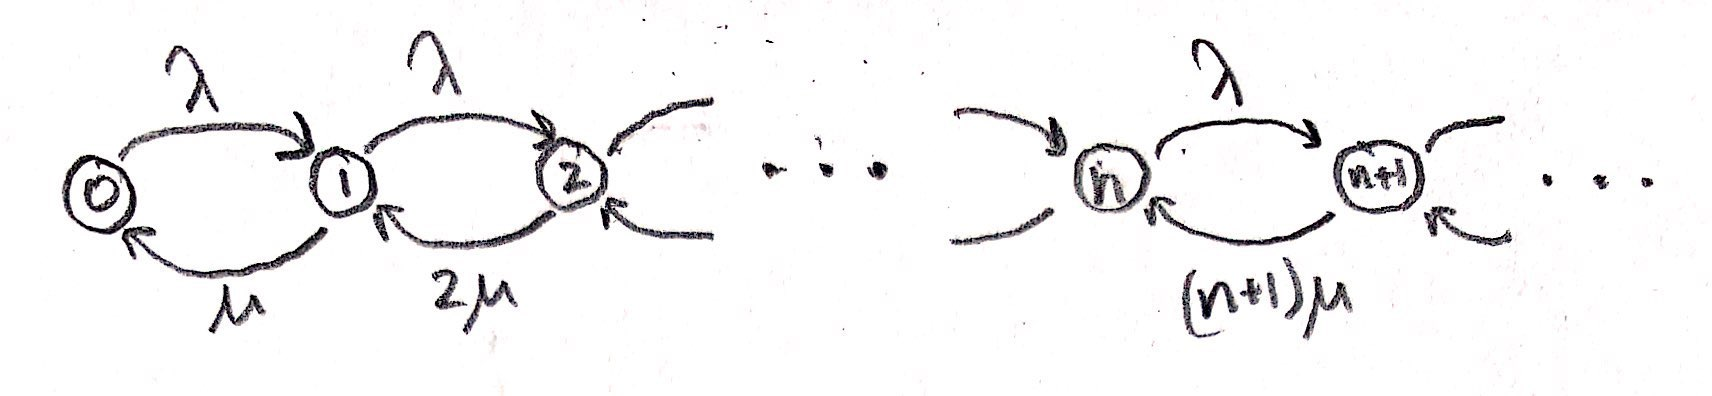
\includegraphics[scale=0.15]{poisson_chain.jpg}
\]

(b) Since an irreducible infinite markov chain is positive recurrent if and only if it has a stationary distribution, it is sufficient to find the stationary distribution. We have the generalized balance equation:
\[
(\lambda + n\mu)\pi_n = \lambda\pi_{n - 1} + (n + 1)\mu\pi_{k + 1}
\]
We claim that $\pi_n = \frac{(\lambda / \mu)^n}{n!}\pi_0$ satisfies these balance equations. Indeed, plugging it in we get equality. Then, normalizing, we get that
\begin{align*}
    \pi_0 &= \frac{1}{e^{\lambda / \mu}} \\
    \pi_1 &= \frac{\lambda / \mu}{e^{\lambda / \mu}} \\
    \pi_2 &= \frac{(\lambda / \mu)^2}{2e^{\lambda / \mu}} \\
        &\vdots \\
    \pi_n &= \frac{(\lambda / \mu)^2}{n!e^{\lambda / \mu}} \\
        &\vdots
\end{align*}
In fact, we note that the number of people in the queue is just $Poisson(\lambda / \mu)$.
\section{Homework 10}
\includepdf[pages=-]{midterm2}

\subsection{Exponential: MLE \& MAP}
(a) We wish to find
\[
\MLE[X | Y] = \argmax_x f(Y | X = x),
\]
so we set derivative to 0,
\[
e^{-xy}(1 - xy) = 0
\]
and find that $\MLE[X | Y] = \frac{1}{y}$.

(b) We wish to find
\[
\MAP[X | Y] = \argmax_x f(x)f(Y | X = x)
\]
so we set derivative to 0,
\[
e^{-(1 + y)x}(1 - x(1 + y)) = 0
\]
and find that $\MAP[X | Y] = \frac{1}{1+y}$


\subsection{BSC: MLE \& MAP}
(a) Let $X$ denote the observation of the input and output. To find MLE of $\epsilon$, we simply compute
\[
\MLE[\epsilon | X] = \argmax_\epsilon \P[X | \epsilon],
\]
where $\epsilon$ is taken over the interval $[0, 0.5]$. Suppose that there are $n$ total bits observed, and $n_e$ of them are corrupted. Then we can find the MLE explicity through
\begin{align*}
    \frac{d}{dx}\left(\epsilon^{n_e}(1 - \epsilon)^{n - n_e}\right) &= n_e\epsilon^{n_e - 1}(1 - \epsilon)^{n - n_e} - \epsilon^{n_e}(n - n_e)(1 - \epsilon)^{n - n_e - 1},
\end{align*}
and so we get
\begin{align*}
    n_e\epsilon^{n_e - 1}(1 - \epsilon)^{n - n_e} &= \epsilon^{n_e}(n - n_e)(1 - \epsilon)^{n - n_e - 1} \\
    \epsilon(n - n_e) &= n_e(1 - \epsilon) \\
    \epsilon &= n_e / n
\end{align*}
for $\epsilon \in [0, 0.5]$.


(b) Let $X_i$ be the input value of the $i$th bit and $Y_i$ be the output value of the $i$th bit. Then we have
\begin{align*}
    \MLE[\epsilon | \vec{X}, \vec{Y}] &= \argmax_\epsilon \prod_{i = 1}^n\P[Y_i | \epsilon] \\
    &= \argmax_\epsilon \prod_{i = 1}^n\left(0.6\P[Y_i | \epsilon, X_i = 1] + 0.4\P[Y_i | \epsilon, X_i = 0]\right).
\end{align*}
Now suppose that $n_0$ of the outputs are 0's and $n_1$ are 1's (so that $n_0 + n_1 = n$). Then our expression becomes
\[
\argmax_\epsilon (0.6\epsilon + 0.4(1 - \epsilon))^{n_0}(0.6(1 - \epsilon) + 0.4\epsilon)^{n_1}
\]
and so we differentiate to get
\[
0.2n_0(0.2\epsilon + 0.4)^{n_0 - 1}(-0.2\epsilon + 0.6)^{n_1} - 0.2n_1(0.2\epsilon + 0.4)^{n_0}(-0.2\epsilon + 0.6)^{n_1 - 1} = 0,
\]
which we solve to get
\[
\epsilon = \frac{3n_0 - 2n_1}{n_0 + n_1},
\]
and of course set it to 0 or 0.5 if this expression goes beyond that range.

(c) Stick the prior distribution of $\epsilon$ into the argmax expression:
\[
\MAP[\epsilon | \vec{X}, \vec{Y}] = \argmax_\epsilon \left((4 - 8\epsilon)\prod_{i = 1}^n\left(0.6\P[Y_i | \epsilon, X_i = 1] + 0.4\P[Y_i | \epsilon, X_i = 0]\right)\right)
\]
Using the same definitions for $n_0$ and $n_1$ for the previous part, we do some algebra (very similar to last part, except the derivative is a bit messier this time), we get:
\[
(8n_0 + 8n_1 + 8)\epsilon^2 + (-28n_0 + 12n_1 - 8)\epsilon + (12n_0 - 8n_1 - 48) = 0,
\]
and from here we can easily plug it into the quadratic formula to obtain the MAP estimate for $\epsilon$.


\subsection{Fun with Linear Regression}
(a) We have that
\[
p(y^{(i)} | x^{(i)}; w) = \frac{1}{\sigma\sqrt{2\pi}}e^{-\frac{\left(y^{(i)} - f(x^{(i)})\right)^2}{2\sigma^2}},
\]
so that the likelihood is
\begin{align*}
    \prod_{i = 1}^np(y^{(i)} | x^{(i)}; w) &= \left(\frac{1}{\sigma\sqrt{2\pi}}\right)^ne^{-\frac{\sum_{i = 1}^n\left(y^{(i)} - f(x^{(i)})\right)^2}{2\sigma^2}}.
\end{align*}

(b) Define:
\[
X = \left[\begin{tabular}{ccc}
--- & $x^{(1)}$ & ---\\
--- & $x^{(2)}$ & ---  \\
--- & $\vdots$ & --- \\
--- & $x^{(n - 1)}$ & --- \\
--- & $x^{(n)}$ & ---
\end{tabular}\right], \quad
y = \left[\begin{tabular}{c}
$y^{(1)}$ \\
$y^{(2)}$ \\
$\vdots$ \\
$y^{(n - 1)}$ \\
$y^{(n)}$
\end{tabular}\right]
\]
We see that with $X$ and $y$ defined this way, the optimal points of
\[
\min_{w \in \R^d}||Xw - y||_2^2
\]
corresponds to the maximizers of the likelihood we calculated in part (a) since $e^{-x}$ is a monotonic decreasing function.

(c) It is similar to the likelihood we calculated in part (a) except with append the Gaussian prior to the product:
\begin{align*}
p(w)\prod_{i = 1}^np(y^{(i)} | x^{(i)}; w) &= \prod_{i = 1}^d\left(\frac{1}{\tau\sqrt{2\pi}}e^{-\frac{w_i^2}{2\tau^2}}\right)\prod_{i = 1}^np(y^{(i)} | x^{(i)}; w) \\
    &= \left(\frac{1}{\tau\sqrt{2\pi}}\right)^d e^{-\frac{\sum_{i = 1}^d w_i^2}{2\tau^2}}\left(\frac{1}{\sigma\sqrt{2\pi}}\right)^n e^{-\frac{\sum_{i = 1}^n\left(y^{(i)} - f(x^{(i)})\right)^2}{2\sigma^2}}.
\end{align*}
Getting rid of constants, we get the unnormalized posterior distribution:
\[
e^{-\left(\frac{\sum_{i = 1}^d w_i^2}{2\tau^2} + \frac{\sum_{i = 1}^n\left(y^{(i)} - f(x^{(i)})\right)^2}{2\sigma^2}\right)}
\]

(d) Define:
\[
X = \left[\begin{tabular}{ccc}
--- & $x^{(1)}$ & ---\\
--- & $x^{(2)}$ & ---  \\
--- & $\vdots$ & --- \\
--- & $x^{(n - 1)}$ & --- \\
--- & $x^{(n)}$ & ---
\end{tabular}\right], \quad
y = \left[\begin{tabular}{c}
$y^{(1)}$ \\
$y^{(2)}$ \\
$\vdots$ \\
$y^{(n - 1)}$ \\
$y^{(n)}$
\end{tabular}\right], \quad
\lambda = \frac{\sigma^2}{\tau^2}
\]
We see that with $X$, $y$, and $\lambda$ defined this way, the optimal point of the problem
\[
\min_{w \in \R^d} ||Xw - y||_2^2 + \lambda||w||_2^2
\]
correspond to the maximizer of the posterior distribution of $w$.


\subsection{Community Detection using MAP}
Let $\Theta$ be the query variable for the communities, and $G$ be the observation of the graph. Also, let $B$ be the set of all bisections of $G$, let $V$ be the vertex set, and let $E$ be the edge set. Then the MAP estimate gives us
\begin{align*}
\MAP[\Theta | G] &= \argmax_{\theta \in B}p(\theta)p(G | \theta) \\
    &= \argmax_{\theta \in B}p(G|\theta) \\
    &= \argmax_{\theta \in B}\prod_{v\neq w \in V}\P\left[\text{``$v$ and $w$ are (dis)connected by an edge in $E$"} | \theta\right],
\end{align*}
where the expression inside the $\P[``\quad"]$ is selected as (dis)connected based on if there is (not) an edge between $v$ and $w$ in the observed graph $G$. It follows that if $\theta$ is selected so that the number of edges that bridge the two communities is the smallest, the expression will be maximized, since $p > q$ and we want more edges (or equivalently, probabilities in the product expression) to be equal to $p$ rather than $q$. Thus the MAP estimate of the two communities is equivalent to finding the min-bisection of the graph.
\section{Homework 11}

\subsection{Flipping Coins and Hypothesizing}
The likelihood function is
\[
L(y) = \frac{f_{Y|X}(y | 1)}{f_{Y|X}(y | 0)} = \frac{(1 - q)^{y - 1}q}{(1 - p)^{y - 1}p},
\]
which is strictly decreasing on $y$ since $q > p$. Thus the solution to this problem can be represented by $\hat{X} = 1\{y < y_0\} + \gamma 1\{y = y_0\}$. Given $\beta$, we maximize $\P[\hat{X} = 1 | X = 1]$ by solving
\begin{align*}
    \beta &= \P[\hat{X} = 1 | X = 0] \\
        &= 1 - (1 - p)^{y_0 - 1} + \gamma p(1 - p)^{y_0 - 1} \\
        &= 1 - (1 - \gamma p)(1 - p)^{y_0 - 1},
\end{align*}
which gives us 
\[
y_0 = 1 + \log_{1 - p}(1 - \beta) - \log_{1 - p}(1 - \gamma p),
\]
where we choose $\gamma \in [0, 1]$ so that $y_0$ is an integer. Thus the solution to our hypothesis testing problem is
\[
\hat{X} = \begin{cases}
1 &\quad\text{ if } y < y_0 \\
1 \text{  w.p. } \gamma &\quad\text{  if } y = y_0 \\
0 &\quad\text{ if } y > y_0.
\end{cases}\]

\subsection{BSC Hypothesis Testing}
Let $Y_1, \dots, Y_n$ be RV's denoting a 1 if bit $i$ was corrupted or a 0 if it was transmitted correctly. Also let $Y = \sum Y_i$, the Then since our likelihood function
\[
L(Y) = \frac{\epsilon'^y(1 - \epsilon')^{n - y}}{(0.1)^y(0.9)^{n - y}}
\]
is increasing on $y$, our solution becomes $\hat{X} = 1\{Y \geq n_0\}$. Applying CLT, we get
\begin{align*}
    \beta &= \P[\hat{X} = 1 | X = 0] \\
        &= \P[Y \geq n_0 | \epsilon = 0.1] \\
        &= \P[\Nor(0.1n, 0.09n) \geq n_0] \\
        &= \P\left[\Nor(0, 1) \geq \frac{n_0 - 0.1n}{0.3\sqrt{n}}\right].
\end{align*}
Given that $\beta = 0.05$, we get
\[
n_0 = 0.1n + 0.495\sqrt{n}.
\]
Thus, the solution is
\[
\hat{X} = \begin{cases}
1 &\quad\text{ if } Y \geq n_0, \\
0 &\quad\text{ if } Y < n_0.
\end{cases}
\]
Indeed, we see that our decision rule is independent of the choice of $\epsilon' > 0$.

\newcommand{\Hi}{\mathcal{H}}
\subsection{Projections}
(a) First, we show that $\Hi$ is a vector space. Let $X, Y \in \Hi$ be random variables with finite second moments. Then $\E[X^2] < \infty$ and $\E[Y^2] < \infty$. Then using Cauchy Schwarz, we have
\begin{align*}
    \E[(X + Y)^2] &= \E[X^2] + 2\E[XY] + \E[Y^2] \\
        & \leq \E[X^2] + 2\sqrt{\E[X^2]\E[Y^2]} + \E[Y^2] \\
        &< \infty.
\end{align*}
Thus $X + Y \in \Hi$, and so $\Hi$ is a vector space. Now, we verify that $\<\cdot,\cdot\>$ satisfies the axioms of an inner product space:
\begin{itemize}
    \item (symmetry) $\<X, Y\> = \E[XY] = \E[YX] = \<Y, X\>$.
    \item (linearity) $\<X + cZ, Y\> = \E[(X + cZ)Y] = \E[XY] + c\E[ZY] = \<X, Y\> + c\<Z, Y\>$.
    \item (positive definiteness) $\<X, X\> = \E[X^2] > 0$ whenever $X$ is not the $\mathbb{0}$ random variable.
\end{itemize}
Thus $\<X, Y\> := \E[XY]$ indeed fashions $\Hi$ into an inner product space.

(b) Let $u, v \in V$ and $c \in \R$. Then we have that
\begin{align*}
    ||(u + cv) - x||^2 &= ||(u + cv) - P_{u + cv}||^2 + 2\<(u + cv) - P_{u + cv}, P_{u + cv} - x\> + ||P_{u + cv} - x||^2 \\
    &= ||(u + cv) - P_{u + cv}||^2  + ||P_{u + cv} - x||^2 \\
    &\geq ||(u + cv) - P_{u + cv}||^2,
\end{align*} 
with equality if and only if $x = P_{u + cv}$. But we also have that
\begin{align*}
    ||(u + cv) - x||^2 &= ||(u + cv) - P_u - cP_{v}||^2 + 2\<(u + cv) - P_u - cP_{v}, P_{u} + cP_{v} - x\> + ||P_{u} + cP_{v} - x||^2,
\end{align*}
and since $U^\perp$ is a subspace, we have $(u - P_u) + (cv - cP_v) \in U^\perp$, and since $P_u, P_v, x \in U$, $P_u + cP_v - x \in U$, so that
\[
\<u + cv - P_u - cP_v, P_u + cP_v - x\> = 0,
\]
continuing, we get
\begin{align*}
    ||(u + cv) - x||^2 &= ||(u + cv) - P_u - cP_{v}||^2 + ||P_{u} + cP_{v} - x||^2 \\
        &\geq ||(u + cv) - P_u - cP_{v}||^2,
\end{align*}
with equality if and only if $x = P_u + cP_v$. But since $x$ was also the minimizer of $(u + cv)$, we see that $P_{u + cv} = P_u + cP_v$. Thus the projection map is linear.

(c) If $\{v_i\}_{i = 1}^n$ is an orthonormal basis, then each of the terms $\<y, v_i\>v_i$ gives the $v_i$-component of the projection in the subspace $U$. To see this, we write it out explicitly as
\[
\<y, v_i\>v_i = ||y||||v_i||\cos\theta_i = ||y||\cos\theta_i,
\]
where $\theta_i$ is the angle between $y$ and $v_i$. Then $||y||\cos\theta_i$ is the length of the projection of $y$ onto the line generated by $v_i$, which is precisely the $v_i$-component of the final projection $P_y$ we want.


\subsection{Exam Difficulties}
(a) After some calculations, we get the following
\begin{align*}
    \E[X] &= 25 \\
    \E[X^2] &= \frac{10000}{9} \\
    \E[\Theta] &= 50 \\
    \E[X\Theta] &= \frac{5000}{3},
\end{align*}
so that using the LLSE formula, we get
\begin{align*}
    L[\Theta | X] &= \E[\Theta] + \frac{\E[X\Theta] - \E[X]\E[\Theta]}{\E[X^2] - \E[X]^2}(X - \E[X]) \\
    &= 50 + \frac{6}{7}(X - 25) \\
    &= \frac{6}{7}X + \frac{200}{7}.
\end{align*}

(b) We have
\[
\MAP[\Theta | X] = \argmax_\theta f_{\Theta}(\theta)f_{X|\Theta}(X|\theta) = \argmax_\theta f_{X | \Theta}(X|\theta) = X.
\]


\subsection{Photodetector LLSE}
Let $X = \Theta + N$, where $\Theta$ is the product of a Bernoulli random variable with parameter $p$ and a Poisson with parameter $\lambda$. Then $X \sim Pois(\lambda)Bern(p) + Pois(\mu)$, so that we get the following calculations necessary for later:
\begin{align*}
    \E[X] &= \lambda p + \mu \\
    \E[X^2] &= p\lambda(\lambda + 1) + 2\lambda p\mu + \mu(\mu + 1) \\
    Cov(\Theta, X) &= Cov(\Theta, \Theta + N) = Cov(\Theta, \Theta) + Cov(\Theta, N) = Cov(\Theta, \Theta) = \lambda^2 p + \lambda p - \lambda^2 p^2.
\end{align*}
Using LLSE formula, we have
\begin{align*}
    L[\Theta | X] &= \E[\Theta] + \frac{\E[X\Theta] - \E[X]\E[\Theta]}{\E[X^2] - \E[X]^2}(X - \E[X]) \\
    &= \frac{\lambda^2 p + \lambda p - \lambda^2 p^2}{\lambda^2 p + \lambda p - \lambda^2 p^2 + \mu}(X - \lambda p - \mu) + \lambda p.
\end{align*}

% \begin{align*}
%     \E[X] &= \lambda p + \mu \\
%     \E[X^2] &= \lambda p(\lambda p + 1) + 2\lambda p\mu + \mu(\mu + 1) \\
%     Cov(\Theta, X) &= Cov(\Theta, \Theta + N) = Cov(\Theta, \Theta) + Cov(\Theta, N) = Cov(\Theta, \Theta) = \lambda p.
% \end{align*}
% Using LLSE formula, we have
% \begin{align*}
%     L[\Theta | X] &= \E[\Theta] + \frac{\E[X\Theta] - \E[X]\E[\Theta]}{\E[X^2] - \E[X]^2}(X - \E[X]) \\
%     &= \frac{\lambda p}{\lambda p + \mu}X.
% \end{align*}
\section{Homework 12}

\subsection{Geometric MMSE}
First, we find the LLSE. We have the following calculations:
\begin{align*}
    \E[N] &= \frac{1}{1 - p} \\
    \E[NT] &= \E[\E[NT|N]] \\
        &= \E[N^2/\lambda] \\
        &= \frac{p + 1}{\lambda(1 - p)^2} \\
    \E[T] &= \frac{1}{\lambda(1 - p)} \\
    Var(T) &= \frac{1}{\lambda^2(1 - p)^2},
\end{align*}
which gives us
\begin{align*}
    L[N | T] &= \frac{1}{1 - p} + \frac{\frac{p}{\lambda(1 - p)^2}}{\frac{1}{\lambda^2(1 - p)^2}}\left(T - \frac{1}{\lambda(1 - p)}\right) \\
        &= \lambda pT + 1.
\end{align*}
Next, we find the MMSE. We have
\begin{align*}
    \E[N | T] &= \sum_{n = 1}^\infty nf_{N|T}(n|T) \\
        &= \sum_{n = 1}^\infty n\frac{\P[N = n]f_{T|N}(T|N = n)}{f_T(T)} \\
        &= \sum_{n = 1}^\infty n\frac{(1 - p)p^{n - 1}\lambda^{n}T^{n - 1}e^{-\lambda T}}{(n - 1)!\lambda (1 - p)e^{-\lambda(1 - p)T}} \\
        &= \sum_{n = 1}^\infty n\frac{(\lambda pT)^{n - 1}e^{-\lambda pT}}{(n - 1)!}.
\end{align*}
Now, if we note that
\[
\sum_{n = 1}^\infty \frac{x^n}{(n - 1)!} = xe^x \implies \sum_{n = 1}^\infty n\frac{x^{n - 1}}{(n - 1)!} = xe^x + e^x,
\]
then we get
\[
\E[N|T] = (e^{\lambda pT} + e^{\lambda pT}(\lambda pT))e^{-\lambda pT} = \lambda pT + 1.
\]
(It's the same as LLSE!)


\subsection{Property of MMSE}
We have that
\begin{align*}
    \E\left[\left(X - \sum_i\E[X|Y_i]\right)\right] &= \E\left[\left(X - \E[X|Y_1, \dots, Y_n] + \E[X|Y_1, \dots, Y_n] - \sum_i\E[X|Y_i]\right)^2\right] \\
        &= \E[(X - \E[X|Y_1, \dots, Y_n])^2] + \\
        &2\E\left[(X - \E[X|Y_1, \dots, Y_n])\left(\E[X|Y_1, \dots, Y_n] - \sum_i\E[X|Y_i]\right)\right] + \\
        &\E\left[\left(\E[X|Y_1, \dots, Y_n] - \sum_i\E[X|Y_i]\right)^2\right].
\end{align*}
Since $\sum_i\E[X|Y_i]$ is in the function space of the $Y_i$, by the orthogonality property, the middle term becomes 0, and our expression simplifies to
\begin{align*}
    &\E[(X - \E[X|Y_1, \dots, Y_n])^2] + \E\left[\left(\E[X|Y_1, \dots, Y_n] - \sum_i\E[X|Y_i]\right)^2\right] \\
    &\geq \E[(X - \E[X|Y_1, \dots, Y_n])^2],
\end{align*}
which was what we wanted.


\subsection{Gaussian Random Vector MMSE}
Since $X$ and $Y$ are jointly gaussian, we have
\[
\E[WX|Y] = W\E[X|Y] = \pm L[X|Y].
\]
Since
\begin{align*}
    \E[X] &= 1 \\
    Cov(X, Y) &= 1 \\
    Var(Y) &= 2 \\
    \E[Y] &= 0,
\end{align*}
we get
\[
    \E[WX|Y] = \begin{cases}
        1 + Y/2 &\f{ if } Y > 0 \\
        -(1 + Y/2) &\f{ if } Y < 0 \\
        0 &\f{ else.}
    \end{cases}
\]


\subsection{Jointly Gaussian MMSE and Correlation Coefficients}
(a) (1) is due to orthogonality property of $L[Y|X]$. (2) follows from (1) since $\E[Y - g(X)]\E[X] = 0$. (3) follows from (2) since for JG random variables, independent is the same thing as uncorrelated. (4) follows from (3) since functions of independent r.v.'s are independent themselves, and thus they are uncorrelated and $\E[(Y - g(X))f(X)] = 0$ for any function $f(\cdot)$. Consequently (5) follows since $Y - g(X) = Y - L[Y|X]$ is now orthogonal to the function space of $X$ and hence $L[Y|X] = \E[Y|X]$.

(b) We have
\begin{align*}
    \rho_1 &= \frac{\E[XY]}{\sigma_X\sigma_Y} \\
        &= \frac{\E[Y\E[X|Y]]}{|X||Y|} \\
        &= \frac{|Y||L[X|Y]|}{|X||Y|} \\
        &= \frac{|L[X|Y]|}{|X|}.
\end{align*}
Similarly
\begin{align*}
    \rho_2 &= \frac{|L[Z|Y]}{|Z|}
\end{align*}
So that 
\begin{align*}
    \rho(X, Z) &= \frac{\E[XZ]}{\sigma_X\sigma_Z} \\
        &= \frac{\E[L[X|Y]L[Z|Y]}{|X||Z|} \\
        &= \frac{|L[X|Y]||L[Z|Y]|}{|X||Z|} \\
        &= \rho_1\rho_2.
\end{align*}

(c) We claim $cor(X_n, X_0) = \pm\prod_{i = 1}^n\rho_i$. By part (b) we get that $cor(X_2, X_0) = \pm\rho_2\rho_1$. By induction on $n$, we see that
\begin{align*}
    cor(X_n, X_0) &= cor(X_n, X_{n-1})cor(X_0, X_{n-1}) \\
        &= \rho_n\prod_{i=1}^{n-1}\rho_i \\
        &= \prod_{i = 1}^n\rho_i.
\end{align*}


\subsection{Stochastic Linear System MMSE}
(a) Since all the gaussians are independent, we have
\[
X_n \sim \mathcal{N}\left(0, a^{2n}u^2 + \sum_{i = 0}^{n - 1}a^{2i}\sigma^2\right) = \mathcal{N}\left(0, a^{2n}u^2 + \frac{1 - a^{2n}}{1 - a^2}\sigma^2\right)
\]


(b) Note that
\begin{align*}
    \E[X_{n+1} | X_n] &= \E[aX_n + V_n | X_n] \\
        &= aX_n.
\end{align*}
So we have
\begin{align*}
    \E[X_{n + m}|X_n] &= a^mX_n.
\end{align*}


(c) We want to have
\begin{align*}
    a^{2n}u^2 + \frac{1 - a^{2n}}{1 - a^2}\sigma^2 &= a^{2n + 2}u^2 + \frac{1 - a^{2n + 2}}{1 - a^2}\sigma^2,
\end{align*}
so we solve for $u$ to obtain
\[
u = \frac{\sigma}{\sqrt{1 - a^2}}
\]


\subsection{Random Walk with Unknown Drift}
(a) In matrix-vector form, the dynamics of the system are:
\begin{align*}
    \left[\begin{tabular}{c} $X_1(n)$ \\ $X_2(n)$ \end{tabular}\right] &= \left[\begin{tabular}{cc} 1 & 1 \\ 0 & 1 \end{tabular}\right]\left[\begin{tabular}{c} $X_1(n-1)$ \\ $X_2(n-1)$ \end{tabular}\right] + \left[\begin{tabular}{c} V(n-1) \\ 0 \end{tabular}\right] \\
    [Y(n)] &= [\begin{tabular}{cc} 1 & 0 \end{tabular}]\left[\begin{tabular}{c} $X_1(n)$ \\ $X_2(n)$ \end{tabular}\right] + [W(n)].
\end{align*}

The recursive equations are:
\begin{align*}
    \hat{X}_{n|n} &= \hat{X}_{n|n-1} + K_n\hat{Y}_n \\
    \Tilde{Y}_n &= Y_n - [1\quad 0]\hat{X}_{n|n-1} \\
    K_n &= \sum_{n|n-1}\left[\begin{tabular}{c} 1 \\ 0 \end{tabular}\right]\left([1\quad 0]\sum_{n|n-1}\left[\begin{tabular}{c} 1 \\ 0 \end{tabular}\right] + [\Nor(0, \sigma_W^2)^2]\right)^{-1} \\
    \sum_{n|n-1} &= \left[\begin{tabular}{cc} 1 & 1 \\ 0 & 1 \end{tabular}\right]\sum{n|n-1}\left[\begin{tabular}{cc} 1 & 0 \\ 1 & 1 \end{tabular}\right] + \left[\begin{tabular}{cc} $\Nor(0, \sigma_V^2)^2$ & 0 \\ 0 & 0 \end{tabular}\right] \\
    \sum_{n|n} &= (I - K_n[1\quad 0])\sum{n|n-1}.
\end{align*}

(b) The prediction gets rid of the noise, so we have
\[
\E[X(n + k) | Y^{(n)}] = \left[\begin{tabular}{cc} 1 & 1 \\ 0 & 1 \end{tabular}\right]^k\hat{X}(n) = \left[\begin{tabular}{cc} 1 & k \\ 0 & 1 \end{tabular}\right]\hat{X}(n)
\]

(c) Eh.



\end{document}
